\documentclass[a4paper,11pt,twoside]{book}
\usepackage[DIV=14,BCOR=2mm,headinclude=true,footinclude=false]{typearea}

\makeatletter
\if@twoside % commands below work only for twoside option of \documentclass
    \newlength{\textblockoffset}
    \setlength{\textblockoffset}{12mm}
    \addtolength{\hoffset}{\textblockoffset}
    \addtolength{\evensidemargin}{-2.0\textblockoffset}
\fi
\makeatother

%Options: Sonny, Lenny, Glenn, Conny, Rejne, Bjarne, Bjornstrup
%\usepackage[a4paper,top=3cm,bottom=3cm,left=3.5cm,right=3.5cm]{geometry}
\usepackage[Lenny]{fncychap}
\usepackage{xcolor}
\usepackage[utf8]{inputenc}
\usepackage[english]{babel}
\usepackage{graphicx}
\usepackage[pdf]{pstricks}
\usepackage{amsmath}
\usepackage{amssymb}
\usepackage[colorlinks=true, allcolors=blue]{hyperref}
\usepackage{hyperref}
\usepackage{pseudocode}
\usepackage{algorithm}
\usepackage{lettrine}
\usepackage[inline]{enumitem}
%\usepackage{draftwatermark}
\usepackage{fancyhdr}
\usepackage{framed}
\usepackage[toc,page]{appendix}
\usepackage{multicol}
\usepackage{graphicx}
\usepackage{subcaption}
\usepackage{booktabs}

\fancyfoot{}
\fancyhead[RO,LE]{\thepage}
\fancyhead[LO]{\leftmark}
\fancyhead[RE]{\rightmark}

\pagestyle{fancy}% Change page style to fancy

\linespread{1.1}

%\SetWatermarkText{DRAFT}
%\SetWatermarkScale{5}
%\SetWatermarkColor[rgb]{0.95,0.95,0.95}
\graphicspath{ {imgs/} }

\begin{document}

\frontmatter 
\pagestyle{plain} 

%------------------------------------------------------------------------------
%	TITLE PAGE
%------------------------------------------------------------------------------

\begin{titlepage}
\begin{center}

\begin{figure}[h]
  \centering
  \includegraphics[width=80px]{upc_logo}
  \label{}
\end{figure}

\vspace*{.02\textheight}
{\scshape\LARGE Universitat Polit\`ecnica de Catalunya\par}\vspace{1.5cm} % University name
\textsc{\Large Master Thesis}
\vspace{1.5cm}
\hrule
\vspace{0.4cm}
{\huge \bfseries Inferring program structure from execution traces\par}
\vspace{0.4cm}
\hrule
\vspace{1.5cm}
 
\begin{minipage}[t]{0.4\textwidth}
\begin{flushleft} \large
\emph{Author:}\\
Juan Francisco Mart\'inez Vera \\
{\tt juan.martinez@bsc.es} % Author name - remove the \href bracket to remove the link
\end{flushleft}
\end{minipage}
\begin{minipage}[t]{0.4\textwidth}
\begin{flushright} \large
\emph{Supervisor:} \\
Jes\'us Labarta Mancho\\
{\tt jesus.labarta@bsc.es} % Supervisor name - remove the \href bracket to remove the link  
\end{flushright}
\end{minipage}\\[3cm]
 
\vfill

\large \textit{A thesis submitted in fulfillment of the requirements\\ for the
degree of Master in Research and Innovation}\\[0.3cm] % University requirement text
\textit{in the}\\[0.4cm]
Performance tools team\\Barcelona Supercomputing Center\\[2cm] % Research group name and department name
 
\vfill

{\large \today}\\[4cm] % Date
%\includegraphics{Logo} % University/department logo - uncomment to place it
 
\vfill
\end{center}
\end{titlepage}

%------------------------------------------------------------------------------
%	QUOTATION PAGE
%------------------------------------------------------------------------------


\clearpage\thispagestyle{empty}\mbox{}\clearpage

\vspace*{0.2\textheight}

{\large \textit{ {\huge ``}Compr\'o Geometr\'ia de Descartes y la ley\'o por si mismo.
Cuando hab\'ia le\'ido dos o tres p\'aginas, se sinti\'o incapaz de seguir
adelante. Empez\'o de nuevo y avanz\'o tres o cuatro p\'aginas m\'as, hasta
llegar a otro punto dificil. Volvi\'o a empezar y avanz\'o un poco m\'as. Y
continu\'o as\'i hasta hacerse dueño de todo su significado.{\huge ''}}}
\begin{flushright}
  Richard S. Westfall -- Isaac Newton: Una vida
\end{flushright}

\clearpage\thispagestyle{empty}\mbox{}\clearpage

%------------------------------------------------------------------------------
%	ABSTRACT PAGE
%------------------------------------------------------------------------------
\chapter*{Abstract}

%HPC has been increasing in importance and nowadays can be said it is the third
%support of science with theory and mathematics. For these systems there is a
%high pressure to be always faster and improvements have been done in all layers
%of the transformation hierarchy. This thesis is centered on program layer and
%the tools that aims to improve execution times here are the performance analysis 
%tools that allows to detect the bottlenecks presents in the application that 
%prevents from better behaviour. In an application-centric approach, the
%performance analysis is a cyclic process consisting of observing the behaviour
%of the application so as to hypothesize the possible problems that affects its
%performance and finally translate these hypothesis to improvements in the
%application, re-starting the cycle to validate them. Obviously as less number of
%iterations of this cycle the less time wasted and it directly depends on the
%quality of the hypothesis that is strongly related with the possibilities the
%analysis tools provides. 

Performance tools have been demonstrated to be valuable
on detection of bottlenecks for a long time but since it demands high skilled
analyst, developers are not used to use them but delegate this work to the
actual specialist. What it means is that analyzers are not used to work with
their own code. Having the structure of the program will lead to better
understand the application by allowing to analyst to have a mental schema about
what the program does. This improve in understandability also will leads to
better and faster analysis while also drives to better reports to the developer. 
Identifying this need, in this thesis we propose a new methodology for
application structure detection. Even if this problem has been previously solved by
different researchers, they used to use sequential pattern mining techniques
what are difficultly scalable what is a big drawback if we pay attention to the
trend of the HPC systems to grow in complexity.
We propose a disruptive design being the key point of the proposal the fact that we
understand this problem
as a classification problem instead of a sequential pattern mining problem. The main
reason to do that is because we are exclusively focused on HPC applications so
we decided to exploit their idiosyncrasy that have leads to a sort of ad-hoc
methodology for HPC application that have allowed to decrease the complexity of
the tool.

A prototype of the proposed methodology have been developed and tested
demonstrating that is scalable and is able to provide correct results for
current real world applications.

%------------------------------------------------------------------------------
%   CONTENT
%------------------------------------------------------------------------------


\tableofcontents
\listoffigures

\mainmatter % Begin numeric (1,2,3...) page numbering
\pagestyle{fancy} % Return the page headers back to the "thesis" style

\chapter{Introduction}

On the context of this thesis the motivations that encourage for this work and
the objectives.

\section{Context}
\lettrine{F}{rom} several decades to nowadays science have been evolving
dramatically in a wide variety of fields, one of the main reasons is because now we
have the technology to provide the enough computational power to face problems
which were typically impossible to solve. The vanguard of this technological
revolution is represented by huge computers with high resources availability
such as processors, memory, disk or network.
In Computer Science the discipline in charge to drive research in this field is 
the High Performance Computing, i.e. HPC. HPC has been increasing in importance 
and nowadays can be said it is the third support of science with theory and 
mathematics. The science that can be done thanks to this big machines goes from 
earthquake predictions to the analysis of the DNA of a carcinogenic cell, from
weather forecast to material physics simulation.

A typical configuration for high performance machines are clusters. It means a 
team of individual processors or multiprocessors (and lately more specific 
hardware like GPUs) working together, interconnected by a super-fast network. 
The fundamental idea behind these big machines is getting speedup by mean of
partitioning the problem and parallelize the execution. So all processors (or a 
subset) in the cluster will be dealing with different parts of the same problem 
and communicating between them in order to end up with a solution. For example 
imagine we have a weather forecast software, in order to speedup the forecast 
we can partition the surface of the earth and hold every portion to one individual
processor. The communications will be needed because the weather will also depend 
on surroundings, so every partition will need also information of other partitions 
results.

\begin{figure}
  \caption{Gordon Moore's prediction done in 1965}
  \label{moore-prediction}
  \centering
    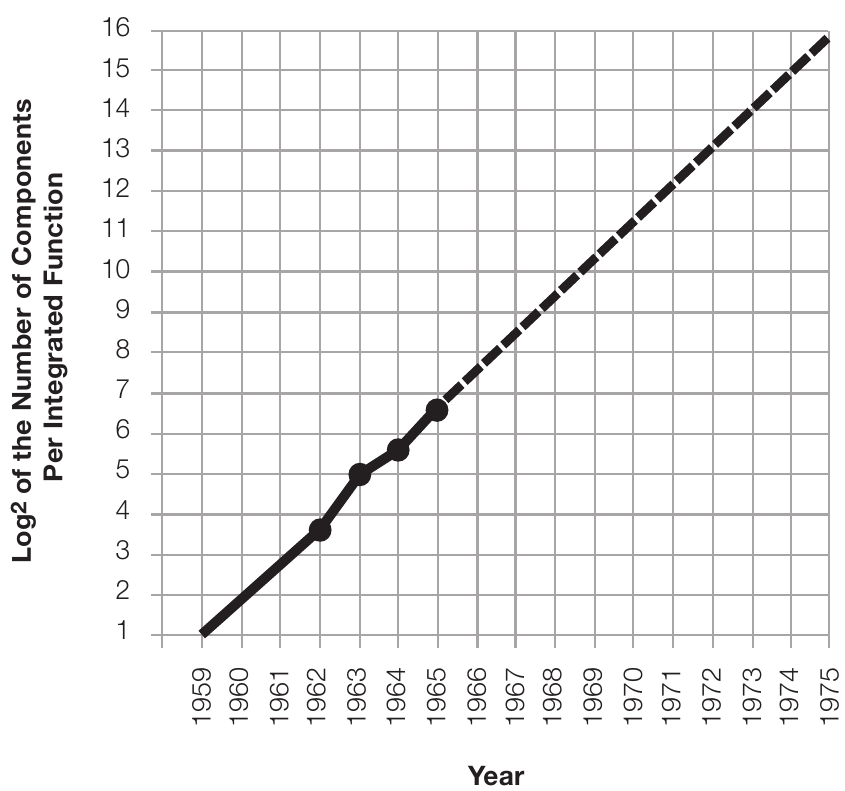
\includegraphics[width=150px]{moore_prediction.png}
\end{figure}


Resources are limited and expensive so we have to use them as efficiently
as its possible. Improving the performance and the efficiency is not just a 
matter that affects to one
layer of the Transformation Hierarchy (proposed by
\cite{transformationHierarchy}, figure \ref{fig:transformation_hierarchy}) 
but can be applied to every one of them. For example the
tremendous evolution of the last fourty years were improvements done mostly on
circuits layer what have been following the Moore's law \cite{moore:1965}. The
manufacturers have been reducing the size of transistors by a ratio of 2 every
18 months as were predicted in figure \ref{moore-prediction}. Performance improvements 
were also at microarchitecture level with
disruptive designs that allows ILP like HPS\footnote{High Performance Substrace,
what is indeed out-of-order execution with in-order retirement.}
\cite{Patt:1985:HNM:18927.18916}, speculative execution with prefetchers, 
branch prediction or even memory access value speculation,
VLIW\footnote{Very Long Instruction Word} or TLP\footnote{Thread Level
Parallelism} with multi-threading. Improvements on memory hierarchy like cache 
associativity, non-blocking cache or trace cache. The last revolution affected 
 microarchitecture, architecture and program layers was the introduction
of multicores (early 2000s). It is basically a revolution in commodity hardware 
because HPC
have been used to use shared memory paradigm for a while like for example with
Convex (1991s). Anyway it is important even in HPC since the trend have
been to move from ad-hoc systems to commodity hardware because the goodnesses of
mass production. On last years researchers have been concerned about the
power consumption because the trend is to have bigger machines so the need of be more
energy efficient is a big deal for the next-generation exascale systems.
Heterogeneity of systems seems to be the trend, i.e. near the typical general
purpose chips install new specific purpose hardware like GPUs or ASICs like
TPUs \cite{jouppi2017datacenter} evolving to an even more complex systems. This
innovation affects to almost all layers of the stack from Program to below. 

\begin{figure}
  \caption{Levels of transformation}
  \label{fig:transformation_hierarchy}
  \centering
    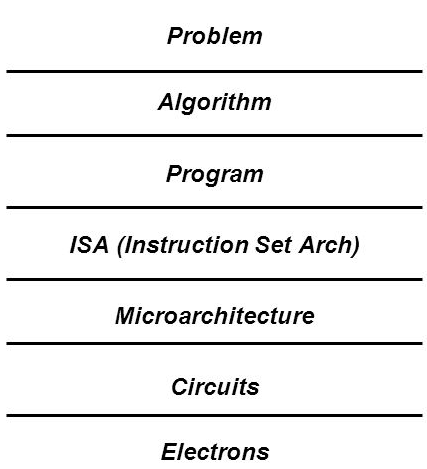
\includegraphics[width=100px]{transformationhierarchy.png}
\end{figure}

Program layer\footnote{The program layer bring together the program itself, 
programming models, frameworks and libraries.} is the interface between pure 
algorithm and the machine architecture. 
It is the actual implementation of the algorithm, i.e. where programmers
transforms algorithm to semantic code that can be transformed lately into
executable binary by compilers. Having an efficient algorithm mathematically 
speaking is not enforcing having an efficient program because at algorithm level 
we do not care about the machine. Pushing on with the business to be always more 
faster and efficient, the tools that aims to this end in program layer are the 
performance analysis tools that allows to detect the bottlenecks presents in the 
application that prevents from better behaviour.

Once the big picture have been briefly introduced now we can zoom in and go a
bit further into details. This thesis belongs to the application performance 
analysis field of research contributing to ease the analysis and the report. 
On the next section a more wide description on performance analysis tools is
presented.

\subsection{Performance analysis tools}

There are two main trends on analysis tools:
\begin{enumerate}[label=\roman*)]
    \item Profiler tools 
      generates performance summaries that provides coarse-grain information, 
      with low-overhead. It is suitable for these analysis where you do not care
      about the fine grain details so you just want a general overview of the
      behavior of the application.
    \item If your goal is to do a fine-grain analysis more detail is needed. The 
      other typical approach are the tracing tools. High accurate and detailed 
      information can be obtained, but it needs more resources in terms of disk 
      and analyst effort because more data implies more complexity.
\end{enumerate}
There is not a general best choice but is just about the needs. One
disadvantage of profiles is that the high degree of aggregation used to hide
variability, for example if there is the case where one single function
behaves different depending on the phase of the execution. In this direction
research has been drived, e.g. phase-base profiling \cite{malony2005phase} or
CCG \cite{knupfer2005construction}. Other one is
that profilers discard the temporal dimension so the execution sequence is lost.
About the advantages, it is a general summary that allows the user to take a
peek about what is going on, e.g. if the user want to speedup a code a profiler
is a good starting point to figure out where to center the efforts. 

If you look
at tracing tools the obvious advantage is that there is a lot of information
available, in fact with not a lot of effort profiler information can be derived
from traces like is done in Cube \cite{saviankou2015cube}. It can be considered
profiler capabilities as a subset of trace analysis capabilities so there should
be a drawback for tracing because tracing is not always the correct choice. The
main drawback is the scalability for both:
\begin{enumerate*}[label=\roman*)]
  \item In tracing time and
  \item in analysis time.
\end{enumerate*}
The problem is becoming worst since the capacity in 
terms of parallelism is increasing\footnote{As have been said High performance 
computers become more complex every generation, e.g. the current number one on 
the Top500 list is the Sunway TaihuLight with 10,649,600 cores\cite{top500_2017} 
.} so the number of tasks to monitor makes 
tracing techniques by one hand hardly scalable and by the other hand tricky to analyze
because the huge quantity of data and because the increasing response times
during the interactive exploration of analysis results. Researchers are currently 
facing the scalability problems in this two forms. 
There are currently several specialists driving research in the tracing
scalability, they are trying to reduce 
the overhead of tracing in terms of time and trace sizes by mean of several 
techniques like machine learning, data-mining and so on like in 
\cite{llort2015intelligent} or by on-line compression like in
\cite{noeth2009scalatrace}. About analysis time, the complexity of the analysis 
can be overcome by adding some sort of automatization. Some examples of this 
research line are automatic performance analysis \cite{wolf2003automatic}, 
automatic structure extraction \cite{casas2007automatic}, phases detection 
\cite{gonzalez2013application} fundamental factors models \cite{casas2008aass}, 
automatic analysis throw deep learning \cite{simon:2017:perfdp} and so on.
Following to this ambition this thesis is focused on the analysis field and is 
devoted to contribute to ease the work of the analyzers by aid part of the analysis. 

\section{Background}\label{s:pt_evironment}

This thesis has been developed in the Performance Tools team at Barcelona
Supercomputing Center and therefore the developments explained in this
document have been designed to fit in this environment, nevertheless the
techniques are general so could be applied to any other environment.

\subsection{Software}

In this section the most important pieces of software used for this thesis
purposes are described. 
%The main tools designed and developed in the BSC 
%Performance Tools Team are Extrae, Paraver and Dimemas although other satellite 
%tools are also in the environment they will not be explained because are out of 
%the scope of this project. These tools are: 
%\begin{enumerate*}[label=\roman*)]
%  \item Clustering
%  \item Tracking
%  \item Folding
%  \item Spectral and 
%  \item Basic Analysis.
%\end{enumerate*}

\subsubsection{Extrae}

Like its name (in spanish) indicates, it is about extracting information. Extrae is
the piece of software in charge of inject monitors to the application to
be studied and
extract valuable information for the analysis. Different mechanism for
monitoring are available being the most used the interposition mechanism by
means of the {\tt LD\_PRELOAD} environment variable present in UNIX systems.
By this mechanism just calls to a given dynamic library can be instrumented because
what it does is to divert shared library calls by the program to extrae, then 
extrae get the information and calls the actual library function. It has the
advantage that the source code is not needed so it can work directly with
already compiled programs without the need of recompile anything. It supports 
several frameworks: 
\begin{enumerate*}[label=\roman*)]
  \item MPI (for several implementations)
  \item OpenMP
  \item OMPSs
  \item CUDA
  \item OpenCL
  \item pThreads
\end{enumerate*}
and virtual machine instrumentation: 
\begin{enumerate*}[label=\roman*)]
  \item Java
  \item and Python.
\end{enumerate*}
The information that can be collected by Extrae is not just timming what is maybe
the most important one but also some hardware counters by means of PAPI
interface. All of this information can be complemented by user events that can
push the desired information to the tracefile by means of the Extrae API. One
possible use of the Extrae API is to extract information about how different
iterations from a given loop are behaving. All these gathered information from 
all threads/processes in the target application is finally merged and presented 
to the analizer as an ASCII tracefile. Since the task of analyze a ASCII file 
is a tough work, a visualizer has been developed, that is Paraver.

The methodology presented in this thesis is about post-mortem trace analysis and
this traces will be generated by extrae so it is an important piece of the
overall workflow. Further Extrae API is used for the validation step in order to
unambiguously detect loops in code and compare the actual structure with the
inferred one automatically without the need of inspect manually the source code.

\subsubsection{Paraver}

The task of analyze raw numbers is tough so the natural choice is to represent 
them visually since we as humans are very
good understanding visual patterns. For example in mathematics
is usual to use plots. In the field of performance analysis, visualizer tools
also has been developed, having in BSC the Paraver (PARAllel Visualization and
Events Representation) tool that as its name indicates
(in spanish) is  about ``to see''. Paraver allows to have a qualitative global 
perception of the application behavior by visual inspection and then to be able 
to focus on the detailed quantitative analysis of the problems.

Its power lies on two main concepts. The first one is that paraver traces are
semantic agnostics therefore it is provided by auxiliar files called pcf (paraver
configuration file\footnote{Do not confuse with cfg files}) and row\footnote{It 
is called row because it provide names for the rows of the timeline so for the 
space axis} (names configuration file). It allows to extend the tool with
support for new performance data or programming models easily. The second and
more interesting is that the derived calculations from initial metrics from trace is
not hardcoded in the tool but configurable so for example to derive a typical
metric like IPC you should filter number of
instructions by one hand, number of cycles by the other hand and then perfom a
division. This powerful approach give the resposability to the user that can
leads to the ``blank page
syndrome''\footnote{https://en.wikipedia.org/wiki/Writer\%27s\_block\#Blank\_page
\_syndrome} for the not so skiled users. For avoid this
sort of problems the Paraver package provides a set of configuration files of
the most used views that perform all the filters and derivations for you.

Even if paraver is not the most important piece of this thesis workflow is
important to introduce it since Paraver traces is what we use and  there is an
interaction between Paraver and the proposed development in the sense that the
second one is capable to identify and communicate with paraver for show up where
in trace are the detected phases.

\subsubsection{Dimemas}

Like the other tools Dimemas also have a so descriptive name, it means (in
spanish) ``tell me more'' but is fine to use the acronym that is ``DIstributed
MEmory MAchine Simulator''. It is a high-abstracted trace-driven MPI simulator
perfect to perform the called ``what if'' experiments. It is capable to simulate
the interconnection network of a distributed memory machine by means of a high
abstracted model that consists on three fundamental parameters:
\begin{enumerate*}[label=\roman*)]
  \item Latency (s) that models the actual latency of the network and also the
    possible overhead because the software stack before arrives to the NIC
  \item Bandwidth (mb/s) that models the bandwidth of the network and
  \item Contention that is modeled by the number of messages in flight 
    allowed on a given instant on a given network (intra-nodes, inter-nodes or
    inter-machines) and the number of input and output messages from a given
    node in a given instant.
\end{enumerate*}

Dimemas works with paraver traces but in this case it needs to perform a 
conversion by {\tt prv2dim} converter that generates a dimemas trace, a
different trace format that ease simulation.
As an output it builds up a
new Paraver trace that can be analyzed as the original. Only communication times 
are simulated through the Dimemas models. Also provides a naive way to model CPU
burst by means of a coefficient that can be applied to their duration.
Additionally ``modules'' can be defined that are segments of the execution where
different coefficients can be applied. Even if it is a minor detail, since it
is important to introduce because its usefulness for this thesis purposes,
there is an additional mechanism to modify CPU burst times. At parsing time
a hardware counter and a coefficient to multiply 
for, can be specified. Normally the hardware counter is the number of 
cycles and the coefficient is the cycle time. By this way the user is able to 
remove the possible O.S. noise that has affected the original
execution\footnote{Noise introduced by O.S. can be detected in Paraver by a fall 
  of the frequency. This is because cycles counter forms part of the context of
  every process but not the time so whenever a process loss CPU, cycles will not
  be counted until return to execution but time is not stopped although. This
  phenomena implies an increment on the traced cycle time. Take into account
  that is impossible to guarantee a fall on frequency is because O.S. or because
  any other source like DVFS so it works only when we can assume the frequency
of the processor is quite stable.}.

Can be considered that Dimemas is completely orthogonal to this thesis objectives
but have been considered interesting to introduce it since in some situations a
Dimemas simulation will be needed in order to remove noise from trace since
noise affects quite enough to the proposed methodology because it rely on some
scalar values like timing instead of just an ordered sequence of events.

\subsubsection{Mercurium}\label{ss:mercurium}

Mercurium\footnote{https://pm.bsc.es/mcxx} is a source-to-source compilation 
infrastructure aimed at fast prototyping. Current supported languages are C, C++
and Fortran. Mercurium is mainly used in Nanos environment to implement OpenMP but
since it is quite extensible it has been used to implement other programming models
or compiler transformations, examples include Cell Superscalar, Software Transactional
Memory, Distributed Shared Memory or the ACOTES project, just to name a few. 

In this thesis it is an important piece since it has been used both for loops
characterization (explained in section \ref{ss:loops_characterzation}) and for
validation phases (explained in section \ref{s:validation}). The reason of use for the former point
is that there were the need of gather information at iterations level and link them
unambiguously to a given loop. This information was impossible to take by means of
typical {\tt LD\_PRELOAD} mechanism so the alternative was to instrument user code and
fire events to trace with the desired information. Since this work is tough when
dealing with large codes, a source-to-source compiler, responsible for doing all the
transformations is ideal. For the validation phase, the reasoning is quite similar but
instead fire hardware information, the automatic code instrumentation just fire loops
boundaries.

There are some other source-to-sorce compiler infrastructures over there like
LVMM\footnote{http://llvm.org/} or Rose\footnote{http://rosecompiler.org/} but finally
Mercurium have been choosen because advantages derived from the proximity since it is
under maintenance and development by the Programming Model team in 
BSC\footnote{https://pm.bsc.es/}.

For more details about the work done with mercurium go to \ref{ann:automatic_code_instr}.

\subsection{Analysis workflow}\label{ss:analysis_workflow}

In an application-centric approach, the performance analysis is a cyclic process 
consisting of observing the behaviour of the application so as to hypothesize the 
possible problems that affect its performance and finally translate these 
hypotheses to improvements in the application re-starting the cycle to validate 
them as is depicted in figure \ref{fig:perf_analysis_workflow}. Obviously, the 
less number of iterations of this cycle the less time wasted and it directly 
depends on the quality of the hypothesis that is strongly related with the 
possibilities the analysis tools provides.

\begin{figure}[]
  \centering
  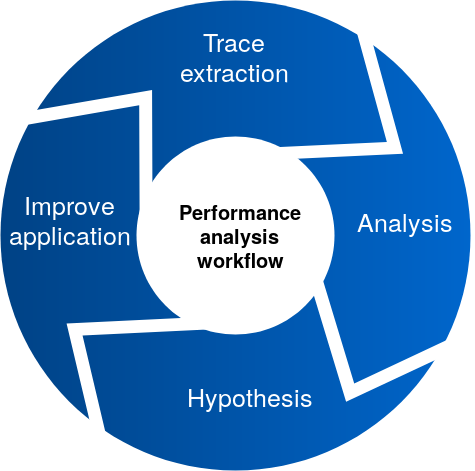
\includegraphics[width=150px]{diagram/performance_analysis_diagram.png}
  \caption{Performance analysis workflow}
  \label{fig:perf_analysis_workflow}
\end{figure}

This work is centered on the analysis phase, so lets go further and look at its
subphases. When dealing with little and medium size traces, visualizers used to
be responsiveness enough to perform analysis directly to the traces but when the 
size surpass a given threshold several previous steps should be done. In last 
cases analysis phase is typically subdivided into the following 
subphases (see figure \ref{fig:analysis_subphases}):
\begin{enumerate}[label=\roman*)]
  \item Before filter phase is
    used to be impossible to work with visualizers so the main goal is to end up
    just with the needed information for inspect the structure of the
    application.
  \item HPC applications are used to have a common idiosyncrasy that is to
    present very repetitive patterns both in space (different processes) and 
    time dimensions. Exploiting this typical characteristic, next step is cut
    the more interesting parts of the execution e.g. an iteration or a set of
    iterations that seems to presents interesting information because its 
    extremely bad performance. This cut is get from the original trace, i.e.
    with all the original information.
  \item Last and most important, the inspection. 
\end{enumerate}

\begin{figure}[]
  \centering
  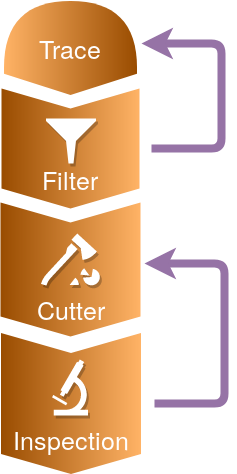
\includegraphics[width=80px]{analysis_subphases.png}
  \caption{Analysis subphases}
  \label{fig:analysis_subphases}
\end{figure}

This work could drive to repeat the same process several times and since every 
one of the steps potentially have a very time consumption, when dealing with
huge trace, it can be a waste of time. 
Both first and second subphases could need to be repeated several times because 
the first filter is not good enough or because on the last phase analyzer realize 
the cut is not as interesting as looked like. The intuition of a high skilled
analyst plays an important role in this process.

As has been covered in motivations (section \ref{s:motivations}) this thesis
approach can be used for improve the inspection subphase but also to help to the
decision or at least give some clues to the analyzer to what region is the most
interesting to cut reducing the number of iterations over the subphases of the
analysis giving more time to the inspection work.

\section{Motivations}\label{s:motivations}

We can say that HPC applications shares a common idiosyncrasy between them. 
Mathematics solvers needs to iterate until the result converge and 
simulation software are used to be programmed to evolve over timesteps. So in 
general, HPC applications consists on a big outer loop that is being executed the 
same code but with evolving data (time axis), and same code with different data
for every parallel process (spatial axis), i.e. SPMD\footnote{Single
Program Multiple Data}. Additionally this kind of workloads are used
to be burst syncrhonous, i.e. all ranks are executing computation and
communication phases in a syncrhonous manner. For these so regular executions a
relatively simple representation of the whole execution could be extracted, i.e.
the trace could be reduced to a minimum pseudo-code expression
with aggregated data for the whole loop so its somehow folding all the iterations
space. This pseudo-code expresses indeed the actual internal structure of the 
application.

There are several factors that motivates for the extraction of the internal
structure of an application being the most important the first one.


\subsection{About improve understandability of execution}

Even if performance tools have been demonstrated to be valuable on detection of
bottlenecks for a long time, since it demands high skilled profiles for the
analysis, developers are not used to use them but delegate this work to the
actual specialist. One example is the POP project\footnote{The POP
  (Performance Optimisation and Productivity) center of excellence in computing
  applications provides performance optimisation and productivity services for
academic and industrial codes in all domains. https://pop-coe.eu/}. What it
means is that analyzers are not used to work with their own codes so they are used
to be agnostics about the structure of the program and it difficults the process
of relate performance metrics to program code. Having the structure of the
program will lead to better understand the application by allowing to analyzer
to have a mental schema about what the program does and allows to relate
differencies in terms on performance to different program phases. This aid on
the understandability will lead to better and faster analysis while also drives
to better reports to the developer.

Profilers are used to present syntactic structure with call path hierarchical 
views where
you can easily pinpoint some aggregated behavioral metrics to a point in
program. Additionally it is a quite scalable solution since the information is
being aggregated during the execution and not big traces are needed. The
counterpart is they present the structure in a static way since they
lost the temporal dimension. It prevents the analyst to have a clear
representation about dynamic execution like loops iterations and they are
exposed just indirectly by the number of calls to a given function. Additionally
some sort of bottlenecks like late-sender problems are difficult to detect. By 
having the syntactic structure that will presents also the temporal order of
things a better understandability of the actual execution can be achieved.

There are previous works (discussed widely on section \ref{related_work})  that 
tries to represent the internal structure of an application but they are used to
use directed graphs like in EFG \cite{aguilar2016event} or just callstack trees like
in Cube \cite{saviankou2015cube}. The drawback of represent the application structure
just with directed graphs is that it is a so simplified view, in the referenced
case it is impossible to pinpoint a given loop (directed graph cycle) to the
actual code because the lack of callstack information. In case of the
referenced approach that uses callstacks tree, the lack of information becomes
from the fact that there is no representation for loops. The identification of 
this lack of clarity
on the structure representation motivates as well this thesis. The proposal is to 
generate a pseudo-code with loop and conditional structures that can be easily 
pinpointed to source code and additionally can show aggregated metrics so it can 
be understood as a sort of mix of the two approaches references above.

\subsection{About identify regions of
interest}\label{ss:mot_regions_of_interest}

The typical tools like visualizers are not enough responsiveness when dealing
with traces with several GB of information so analysts needs to first
preprocess the trace before go ahead with the actual inspection. This preprocess
consists basically on filter and cut the trace (widely explained on
\ref{ss:analysis_workflow}) for identify and inspect just these interesting 
hotspots where the bottlenecks seems to be. Automatically extract the structure
of the application will give the possibility to agregate information by phases
and loops so it can aid to analyzer into the work of find out the
hotspots. In this paper \cite{trahay2015selecting} they present an automatic
tool that extract this points automatically based on the criteria that
iterations that behave different from the mean are the interesting ones. The
problem with the approach presented on the cited paper is that the methodology
is difficultly scalable since it presents high complexity and is I/O
intensive since the data should be readed repeatedly and it is a problem
when dealing with big traces. 

\subsection{About been scalable}

Current approaches about extract the intern structure (syntactic but not
behavioral, more details in \ref{related_work}) based on a post-mortem trace
analysis rely on pattern mining techniques (the basic idea of these algorithms 
are exposed on section \ref{pattern_mining}) that is the obvious choice because 
a trace is basically a sequence of events sorted by time. The problem with these 
sort of algorithm is the complexity. So the last motivation is about reducing the 
complexity of this task. The performance of the proposed algorithms are
prohibitive like in \cite{trahay2015selecting} \cite{Safyallah2006}
\cite{Lopez-Cueva2012} so taking into account the exponential increassing of 
traces sizes this thesis contribution is the idea to perform intern structure 
analysis instead of as a pattern mining problem, as a classification problem. 
Classification algorithms like clustering presents about quasy-lineal costs.


\section{Expectations}

The goal of this work is to automatically detect the internal structure of an 
application and correlate it with performance metrics by mean of a post-mortem 
trace analysis that will help to have a general overview about the phases of the 
execution. This will allow the analyst to build up a mental schema about the
application and understand more easily what could be going on. Furthermore it will 
contain source code information that will allow to easily pinpoint one metric to 
the actual code providing an enhancement on the analyst-developer
understanding. Additionally this structure extraction can help the analyst to 
decide what part of the trace analyze first since it will allow to know the loops 
and iterations boundaries.

The main objective is to detect those sets of events in trace that are being
repeated together several times (above a given threshold) and group them into 
loops. Since several subsets can appear because an application used to have 
dozens of loops, those detected events subsets also will be arranged (in a 
hierarchical manner) in a way that represents faithfully the actual internal 
structure. This sort of analysis have been done typically by using sequential 
pattern mining techniques what is in principle the set of techniques that better 
fits to this problem since a trace is just a sequence of events ordered by time.

Based on previous works and on the premise that HPC applications used to present
the same idiosyncrasy (SPMD, burst synchronous,\ldots) has been decided to
explore a new way to detect those patters, motivated mainly for the fact that
pattern mining techniques are in general computationally expensive. By using data 
mining clustering techniques we expect to have an scalable
solution since it is used to present quasy-lineal complexity with the number of 
elements to clustering. The mapping between elements to clustering and events on
a trace is not bijective but exhaustive, so every element potentially represents 
several trace events, what is in fact the same instruction presenting its dynamic
aspect because the execution of loops. Further the reduction of the tracefile
events to the set of elements to clustering is not needed to be sequential but 
can be done in parallel by splitting the trace into several files and process
them by multiple processes (assuming also multiple HDDs). Assuming repetitive 
executions, the number of elements to clustering would be about constant despite 
the increasing of the execution time.

In this work is not expected to end up with a completely functional and
performance refined tool but demonstrate how this approach can present valuable 
results with a good scalability on increasing trace sizes.

\chapter{State of the Art review}

On how the pattern mining techniques has been the typical algorithms used for
structure detection on the performance analysis field. Before entering to the 
state of the art have been considered interesting to introduce briefly the 
fundamentals on pattern mining techniques for better understanding.

Traces are basically logs that gather information of the execution of an
application. In a more abstract way, we can define traces just as a sequences
of time ordered events. The fundamentals of recognize the intern structure of an
application is about recognize loops that are those structures in code that
repeats the code into their body as many times as programmer want. Loops in
traces has been unrolled and presents its dynamic aspect so we can define loops
as a sub-sequences of instructions that are repeated several times. The work of
identifying loops in traces is about identifying these repetitive sub-sequences.

\section{Sequential pattern mining}\label{pattern_mining}

\lettrine{S}{equential} pattern mining can be defined as: \textit{``Given a set of data sequences, the
problem is to discover sub-sequences that are frequent, that is, the percentage of
data sequences containing them exceeds a user-specified minimum support.''}. Note 
this definition fits pretty well with our objective of loops recognition in traces 
so sequential pattern mining is the natural choice. Furthermore there is another
definition that fits even better for our problem. It is, referring to patterns to
analyze in a temporal sequences:\textit{``\ldots a collection of events that
occur relatively close to each other in a given partial order, and \ldots
frequent episodes as a recurrent combination of events''}.

Sequential pattern mining is a technique applied on a wide range of problems
like for example predicting systems failure by analyzing a sequence of logs,
characterize suspicious behaviour in users by analyzing the sequence of commands
entered, for automatically determine “best practices” by analyzing the sequences
of actions of an expert, etc so the evolution on this area has been quietly
ad-hoc to every problem. On this section pattern mining is introduced and three
main classes of algorithms are explained always from an abstracted point of
view, i.e. without entering into details for specific implementations. This
explanations were taken from \cite{mooney2013sequential}. Even if the temporal
sequences algorithms described in section \ref{ss:temporal_sequences} seems to
be the better choice for structure detection, it has been considered to explain
briefly the other types since most of the ideas were first proposed by them.

\subsection{Formal notation}\label{ss:formal_notation}

Items are literals that belongs to a given alphabet $I=\{i_{1}, i_{2}, \dots,
i_{m}\}$. Then an event is stated as a non-empty unordered set of items
$(i_{1}, i{2}, \dots, i_{k})$. Finally a sequence is an ordered list of
events $\langle\alpha_{1} \rightarrow \alpha_{2} \rightarrow \dots \rightarrow
\alpha_{q}\rangle$. The ordered metric can be time, space or other. When a
sequence is refered as a $k-sequence$ means that this sequence contains $k$
items. A sequence $\langle\alpha_{1} \rightarrow \alpha_{2} \rightarrow \dots 
\rightarrow \alpha_{n}\rangle$ is a subsequence of $\langle\beta_{1} \rightarrow 
\beta_{2} \rightarrow \dots \rightarrow \beta_{m}\rangle$ if there exists
integers $i_{1}, i_{2}, \dots i_{n}$ s.t. $\alpha_{1} \subseteq \beta_{i_{1}}, 
\alpha_{2} \subseteq \beta_{i_{2}}, \dots, \alpha_{n} \subseteq \beta_{i_{n}}$.
So for example $\langle B \rightarrow AC\rangle$ is a subsequence of 
$\langle AB \rightarrow E \rightarrow ACD \rangle$ being the set of integers 1
and 3.

Having a set of sequences $D$, {\it support} or {\it frequency} of a sequence,
denoted as $\sigma(\alpha, D)$, is defined as the number of input sequences in $D$
that contain $\alpha$. A sequence is {\it frequent} or not depending on a
threshold named {\it minimum support}, so is frequent if it happens more than
{\it minimum support} times. The set of frequent k-sequences is denoted as
$L_{k}$. Moving on, a frequent sequence is {\it maximal} if it is not subsequence
of any other frequent sequence. The task becomes to find all maximal frequent
sequences from $D$.

% REMOVE ?????
%This definition is a general abstracted definition and can be adapted for
%ad-hoc algorithms so for example for the topic we are aware of, items can be the
%MPI calls. In this case the
%definition of subsequence can be transformed to “if there exists integers 
%$i_{1}, i_{2}, \dots i_{n}$ s.t. $\alpha_{1} = \beta_{i_{1}}, 
%\alpha_{2} = \beta_{i_{2}}, \dots, \alpha_{n} = \beta_{i_{n}}$” because all
%events are sets of one item. If we use the whole callpath instead of just the
%MPI call and items are the different calls, now events can not be unordered set
%of items but ordered. 
% ????????????

\subsection{Apriori-based algorithms}\label{ss:apriori_based}

Mining frequent itemsets is the core of later analysis like mining association
rules, correlations, sequential patterns and so on. Apriori first proposal was
about discover intra-transaction associations used
in database mining, also called knowledge discovery.
Being $I=\{i_{1}, i_{2}, \dots,i_{m}\}$ a set of literals called items and T a
transaction $T \subseteq I$ is said T contains X if $X \subseteq T$. Further, an
association rule is an implication of the form $X \Rightarrow Y$ where $X
\subset I$, $Y \subset I$ and $X \cap Y = \emptyset$. Apriori algorithm was
presented in the following paper \cite{agrawalfast}. The basis of this algorithm
is presented here and several later algorithms were based on this like for
example AprioriAll, AprioriSome, DynamicSome, GSP (Generalized Sequential
Patterns), PSP and so on. Every one of them are introducing several
optimizations and varying mainly the candidates generation step (explained on
section \ref{ss:discovering_large_itemsets}) but maintains 
the basic core.

The algorithm consists on two fundamental steps being the first the most
challenging one:
\begin{enumerate}
  \item Find all sets of items (itemsets) that have transaction support above
    minimum support.
  \item Use the large itemsets (itemsets above minimum support) to generate the
    desired rules.
\end{enumerate}

\subsubsection{Discovering large itemsets}\label{ss:discovering_large_itemsets}

The large itemsets discovering implies several passes over the data. The first
pass is to find out individual items that are actually large, so which of them
appears more than minimum support. 
On next pass these large items are the seeds, with these
seeds the candidate itemsets are generated and the data is passed again in order 
to find out the large itemsets among the candidates. The same process is repeated 
until no new large itemsets are found. The basic intuition is that any subset of
a large itemset must be large. The algorithm looks like as in pseudocode
\ref{pc:apriori}.

The key point in this algorithm is the candidates generation. It is formed by
two steps. The first step is to generate all the candidates and the second is to
prune those candidates that for sure will not be large itemsets. First step is
represented in pseudocode \ref{pc:apriori_candidate_generator1} and it can be
seen that seed itemsets (from previous pass) are merged in pairs by adding last
item from first itemset to the second. Last phase depicted in
\ref{pc:apriori_candidate_generator2} is about prune the candidates
that contain (k-1)-itemsets that do not exists on $L_{k-1}$. The idea behind
that is what has been exposed before, i.e. any subset of a large itemset must
be large. This property leads to a powerful pruning. By doing that, the 
number of candidates is reduced considerably. By this approach is achieved 
that $C_{k} \supseteq L_{k}$. Ideally $C_{k} = L_{k}$
so as better the candidates generation is, less verifications (whether the minimum
support is achieved or not) will be done and so better performance.

\begin{pseudocode}{Apriori algorithm}{D}
\label{pc:apriori}
    L_{1} \GETS large \quad 1-itemset
	\\
    \FOR k=2; L_{k} \neq \emptyset; k++ \DO
	\BEGIN
        \COMMENT{New candidates} \\
        C_{k} \GETS aprioriGen(L_{k-1})\\
        \FORALL transactions \quad t \in D \DO
        \BEGIN
            \COMMENT{Candidates contained in t} \\
            C_{t} \GETS subset(C_{k}, t)\\
            \FORALL candidates \quad c \in C_{t} \DO
            \BEGIN
                c.count++\\
            \END\\
        \END\\
        L_{k} \GETS \{c \in C_{k} \mid c.count \geq minsup\}
	\END\\
	\\

    \RETURN \bigcup_{k}L_{k}
\end{pseudocode}

\begin{pseudocode}{Apriori Candidate Generator 1}{L_{k-1}-itemsets}
\label{pc:apriori_candidate_generator1}
\text{ {\bf insert into}} \quad C_{k}\\
\text{ {\bf select}} \quad p.item_{1},\ldots,p.item_{k-1},q.item_{k-1}\\
\text{ {\bf from}} \quad L_{k-1} \quad p,L_{k-1} \quad q\\
\text{ {\bf where}} \quad p.item_{1},\ldots,p.item_{k-2} = q.item_{k-2}, 
p.item_{k-1} < q.item_{k-1}\\
\COMMENT{Last condition is for ensuring no duplicates}
\end{pseudocode}


\begin{pseudocode}{Apriori Candidate Generator 2}{L_{k-1}-itemsets, C_{k}}
\label{pc:apriori_candidate_generator2}
    \FORALL itemsets \quad c \in C_{k} \DO
    \BEGIN
        \FORALL (k-1)-subsets \quad s \in c \DO
        \BEGIN
            \IF s \not\in  L_{k-1} \THEN
                delete \quad c \quad from \quad C_{k}\\
        \END
    \END
\end{pseudocode}

%Names used to be so descriptive and therefore can explain quite a lot about the
%reality of the entity. Apriori meaning (by oxford dictonary) is {\it “using facts or
%principles that are known to be true in order to decide what the probable
%effects or results of something will be [\dots]”}. In this case, the name comes
%from the generation-and-test technique. A priori, all candidates formed by
%(k-1)-itemsets combinations are k-itemsets but it have to be tested.

\subsection{Projection-based pattern growth
algorithms}\label{ss:projection_based}

Candidates generation presents to be critical for apriori algorithms and even if
optimizations in the prune process has been introduced, the generated candidates
follows an exponential grow. For example for detect a maximal sequence of 100
elements, $2^{100} \approx 10^{30}$ candidates will be generated. The next
problem is that for every step, data needs to be revisited to check out whether 
new candidates are large itemsets or not. 

Pattern growth paradigm presented in \cite{han2000mining1} remove
completelly the necessity of candidates generation. They achieve improvements on
performance for about one order of magnitude respect Apriori-like algorithms
explained on previous section by adding two key concepts. 
\begin{enumerate*}[label=(\roman*)]
  \item Frequent pattern tree or FP-tree for short
  \item and FP-tree based pattern mining called FP-growth.
\end{enumerate*}
Following, this two concepts are explained in more detail.

\subsubsection{Frequent pattern tree}\label{ss:frequent_pattern_tree}

The following observations can be used for introduce FP-trees and have been used
for its construction. This structure dramatically decrease the size of data to be 
scanned but maintains all the need information for the mining.

\begin{enumerate}[label=\roman*)]
  \item One important rule learned from apriori approach is that frequent
    $(k+1) itemsets$ only can be done from frequent $(k-1) itemsets$. This observacion
    leads to the idea of just taking into account frequent $(1) itemsets$ given a
    minimum support.
  \item These discovered frequent intemsets could be stored in some compact
    structure, avoiding repeatedly scanning the DB.
  \item Continuing with the idea of compacting important data, it can be said
    that identical frequent itemsets from different transactions can be merged
    into one with information about number of occurrences.
  \item And for these partially identical frequent itemsets, shared prefixes can
    be merged as well.
\end{enumerate}

For improve understandability lets drive a construction of an FP-tree following an
example. Imagine we have a database with several transactions like the depicted
in figure \ref{fig:fp_tree_db} (left hand side column). The process ends up with
Fp-tree in figure \ref{fig:fp_tree_constructed}. Lets see how it happens. 

First scan of database derives a list of frequent items, i.e. these 1-itemsets 
above the minimum support value (3 for this example) that is $\langle
(f:4),(c:4),(a:3),(b:3),(m:3),(p:3) \rangle$. Note the frequent items in every
transaction are on right hand side column in figure \ref{fig:fp_tree_db}. The
frequent itemsets here are not sorted by appearance in transaction but by
frequence. This sorting will allows more compression on FP-tree construction. The 
second scan is done over these frequent 1-itemsets and drives the
FP-tree construction. First transaction leads to the construction of the first
branch (left hand side). Next transaction shares the three first items, so
it can be partially merged with first branch. The merge process is just about
update the counters and make the new relations. Same process for all
transactions. Additionally to the pure tree construction, header table structure 
is done for ease the task of traverse all possible frequent patterns that 
contains a given item. 

\begin{figure}
  \centering
  \includegraphics[width=250px]{fp_tree_db}
  \caption{A transaction database as running example}
  \label{fig:fp_tree_db}
\end{figure}

\begin{figure}
  \centering
  \includegraphics[width=200px]{fp_tree_constructed}
  \caption{The FP-tree}
  \label{fig:fp_tree_constructed}
\end{figure}

\subsubsection{Mining FP-trees}

After prepare data FP-growth algorithm is the responsible to find out the
frequent patterns by analyzing the FP-tree. The mining starts with 1-itemset
analysis. Thanks to the header table all paths for a given item $a_{i}$ can be get
easily. Once all paths, where the given item is involved on, are retrieved a new 
subtree is build up. Remember that in this process all items below minimum support 
are pruned. Unlike before now only these retrieved items are taken into account 
for the counting. This new structure is named $a_{i}$ conditional pattern base,
i.e. the sub-pattern base under the condition of $a_{i}$ existence. Next step is
to call mining function recursively having on every recursive call a large
conditional pattern base, so it is growing. It can be better understood by means
of an example. Lets follow the previous one.

Starting from the bottom of the header table, lets mine FP-tree for the $p$ item. Two
paths arise: $\langle f:4,c:3,a:3,m:2,p:2 \rangle$ and $\langle c:1, b:1, p:1
\rangle$ (being the number after ``:'' the occurrences). Note that even if $f$
appears 4 times, only 2 of them appears with $p$, so the path becomes $\langle 
f:2,c:2,a:2,m:2,p:2 \rangle$. Similarly with second path. Moving on, the
construction of the $p$ conditional pattern base is done by counting and pruning
these items below minumum support (3 for the example), so the only branch for the new FP-tree is
$(c:3)$. Hence only one frequent pattern is derived, i.e. $(cp:3)$. From now to
the end, $p$ does not need to be taken into account any more, this is because
all possible patterns containing $p$ has been already analyzed. Similarly we can proceed analyzing paths containing $m$ item. Two paths arise: 
$\langle f:2,c:2,a:2,m:2 \rangle$ and $\langle f:1,c:1,a:1,b:1,m:1 \rangle$. The
new conditional FP-tree just contains the path $\langle f:3,c:3,a:3 \rangle$.
For show how the pattern is growing, lets see in a deph-first way what
recursive calls are done:
\begin{enumerate*}[label=(\roman*)]
  \item mine($\langle f:3,c:3,a:3 \rangle \text{\textbar} m$)
  \item mine($\langle f:3,c:3 \rangle \text{\textbar} am$)
  \item mine($\langle f:3 \rangle \text{\textbar} cam$)
\end{enumerate*}
The frequent pattern derived from this analysis is $(fcam:3)$.

\subsection{Temporal sequences}\label{ss:temporal_sequences}

In this section will be shown the basis of these algorithms that concers about
the periodicity of a certain patterns over the time (generalizing, over any
metric from which the sorting is done). These are obviusly the
algorithms that best fits to the needs for trace structure detection. First
developed framework for datasets considered to be episodic was presented by
\cite{mannila1995discovering}.

Two previous approaches were concerning about the analysis of arbirary ordered
sequences of data, however, this approach considers order as an inherent
characteristic of the sequential structure. This main difference leads to a
slightly different approach of sequential pattern mining and introduce new ideas 
like sliding windows. Nevertheless some important components are shared among 
them like:
\begin{enumerate*}[label=(\roman*)]
  \item Frequency threshold, that is defined as the minimum number of times a
    sequence have to appear. It is analogous to minimum support of apriori and
    pattern-growth algorihtms.
  \item Relies on generate-and-test paradigm to discover frequent sequences. It
    is same approach like apriori-like algorithms.
  \item Finnaly also takes profit from the principle of: all subepisodes are at
    least as frequent as the superepisode, for candidates generation.
\end{enumerate*}

The main objective of these sort of algorithms is: Given a class of episodes, an
input sequence of events, a window width, and a frequency threshold, find all
episodes of the class that occur frequently enough. Before go to the actual 
algorithm let's take a look to the main concepts.

\subsubsection{Temporal sequences formal notation}

On section \ref{ss:formal_notation} have been shown the typical formal notation
for pattern mining, now this notation is extended for explaining the new
concepts that arise from the temporal sequences minning.

Given a class of elementary event types $E_{0}$, an event is a pair $(e,t)$
where $e \in E_{0}$ and $t$ is an integer that represents the instant when
the event appears. An event sequence is a triple $S=(T_{s},T^{s},S)$ where
$T_{s}$ is the starting time, $T^{s}$ is the closing time and $S$ is an ordered
sequence of events.

A windows on $S=(T_{s},T^{s},S)$ is a sequence of events $W=(T_{w},T^{w},W')$
where $T_{s} \leq T_{w}$,$T^{w} \leq T^{s}$ and $W'$ consists on those events
$(e_{i},t_{i})$ where $T_{w} \leq t_{i} < T^{w}$. The width of windows is
$width(W)=T^{w}-T_{w}=w$ and the set of all windows in a sequence S is
$aw(S,w)$. Episodes are collections of events occurring frequently 
close to each other, in
general, are partially ordered sets of events that can be described as a
directed acyclic graph. Are denoted as $\varphi =(V,\le,g)$ where V is a set of
nodes, a partial order $\le$ on V and a function $g:V \rightarrow E_{0}$
associating each node with an event type. In general V also can contain other
episodes forming composite episodes. Episodes can be parallel or sequential.
Is parallel when the partial order relation is trivial and an episode is
sequential if the partial order relation is a total order. The crucial
observation is that all episodes can be described as a composition of parallel
and sequential episodes. Last definition is the episode frequency that 
is described as the ratio between the number of windows containing a given 
episode and the total number of windows:
$$
fr(\varphi,S,w)=\frac{|\text{\{}W \in aw(S,w) | \varphi \text{ occurs in }
W\text{\}}|}{|aw(S,w)|}
$$
So an episode is said to be frequent if $fr(\varphi,S,w)$ is above $min\text{\_}freq$
that is provided by the user.

\subsubsection{Algorithm}

First step is to finding all frequent episodes in the given sequence, given a
class of episodes and a frequency threshold. This part is just like apriori
algorithm. The basis of the algorithm presented here is shared with the already 
presented in section \ref{ss:apriori_based} in the sense that they are based on an
iterative process that consists on an alternation between building candidates 
and recognize frequent episodes by scanning the input data. There is a detail
here that makes this phase potentially outperform the naive Apriori-like
algorithm. Now we are working with windows, and we consider just patterns than
fits on windows so there is a non-sense to try to get $k-itemsets$ having $k >
w$ so the search space is pruned by the windows size. Once all frequent 
episodes are taken then the second step is about recognizing episodes in 
sequences. The entire sequence is traversed by a sliding windows and for every one of these windows the analysis looking for episodes is done. 
Different methods are used for the detection. 
\begin{enumerate}[label=\roman*)]
  \item Parallel episodes: For candidate parallel episode there is a counter
    that indicates how many events of episode appears into the windows. If the
    counteris equal to $|\varphi|$ the index of windows is saved because it
    indicates, the episode has been detected. When the counter is decremented
    it means that we can add one more windows where this episode is.
  \item Serial episodes: Serial candidat episodes are recognized by using state
    automata. A new instance of the automata is initialized whenever first event
    of episode appears on the sliding windows. This automata reach the accepting
    state when all events are present (and have been arising following a certain
    order) and is deactivated when the first element
    that motivates its activation leaves the window. When an automata is removed
    and there is no other automata for this episode, the number of occurrences
    is incremented.
\end{enumerate}

Instead of applying a naïve approach where every windows is scanned
completelly, episodes are recognized in sequences in an incremental fashion. 
Two adjacent windows are typically very similar so after
recognizing episodes in a windows, incremental updates in data structures can be
done for the next one.

Like previous algorithms, the exposed above is just he basic idea and more
research has drive to better algorithms but maintaining this fundamental idea.
Important to mention the Projected Window List presented in
\cite{huang2004prowl} that it use a sort of pattern-growth fashion for temporal
sequences mining for avoid candidate generation.


\section{Previous and related work}\label{related_work}

\lettrine{S}{everal} tools are actually being used in order to ease the analyst
work. Talking about structure analysis we can split previous works into two main
subsets. By one hand we have the behavioral structure that want to expose the
different phases on an execution in terms of performance and by the other hand
the syntactic structure that provide information about the actual program
structure.

\subsection{Behavioral structure}\label{ss:behavioral_structure}

If we consider the same bunch of code will behave, in general, in the same
manner it can be assumed that there is a powerful correlation between the
behavior and the code. By this way it can be said a behavioral analysis is a
side-channel analysis because indirectly the internal syntactic structure can be
betrayed. This consideration could be true in some cases but not in others so the 
main goal of the different approaches presented in this section is not
to present a syntactic but a behavioral structure. The motivation is that when
analyst deals with syntactic structure, like in profilers, time variations of 
the same functions is
hidden, this situation can appears for example when calling same function with
different parameters. For the analyst point of view could be more interesting to
have this information unfolded. Take into account that this same property can
end up identifying different parts of the code as the same phase.

Even if the goal of the approaches explained below does not match perfectly with
goal of this thesis, they provide a really useful insights as a related work.

In \cite{casas2007automatic} they propose 
automatically extract the internal structure of an MPI application from a
Paraver tracefile and provide to analyst just representative phases and they 
rely on signal analysis for this propose. 
Their analysis consists on two main steps:
\begin{enumerate*}[label=\roman*)]
    \item The first is to clean-up the trace by identify the perturbed regions.
Perturbed regions are those parts of the trace that has been perturbed nor by
the application nor by architecture but by external factors such that unknown
system activity or tracing package. Their clean-up phase is centered on remove
noise from tracing package, i.e. flush to disk. By building up a signal based
on flushing events and transform it by Closing morphological filter they end up
with this perturbed phases. 
    \item The second step is the identification of the
phases. It is done by means of autocorrelation and periodicity analysis of a
signal. This signal is build up from any metric like instantaneous FLOPs but
they use number of MPI point to point calls being executed. Once the period is
successfully detected the same process is done recursively on one of the
periods. This allows to have a hierarchical structure. 
\end{enumerate*}
Finally the output is
basically information about the different phases like number of iteration and
timing plus some representative cuts of the original trace. 

In \cite{gonzalez2013application} propose a
technique to identify the different execution phases using clustering 
techniques. Different parts of the
execution are considered as the same phase depending on the behavior,
so an analysis using some hardware metrics is
performed. The first step is about reducing the complexity of the clustering by
filtering the less relevant computation burst, i.e. little bursts according
with a given threshold. The second step is the clustering itself made with the 
CPU burst with hardware counters information attached. In order to 
reduce the dimensionality the proposal is to
use two different dimension sets: The first one is Completed Instructions
against IPC\footnote{Instructions per cycle}. This configuration provides a
performance view. The second is Completed instructions against L1 and L2 cache
misses. This combination reflects the impact of the architecture on the
application structure. Once the CPU burst have been clustered, this information
can be sent back to the trace and can be visualized by the analyst. Additionally
an interesting analysis can be done with the shape of clusters like for example,
working with IPC vs. Number of instructions if the shape of a given cluster is
flat on the second axis it means that there is an imbalance on instructions.
Clustering in the field of performance analysis was used before this proposal 
just for classify processes that behaves similar so its utilization by
identifying different phases on temporal dimension opened the door to new research
paths.

\subsection{Syntactic structure}\label{ss:syntactic_structure}

%Syntactic structure is centered on providing the actual program code structure so
%it needs to use some debug information about symbols and about the position of
%the instruction is being executed, i.e. the callstack.

One of the main interest on having the syntactic structure of an application is to be
aware about not just what but where. This is important in the process of who to
blame in code and provides insights of the actual application that with just
behavioral structure can not be presented like for example where do we have
loops and how many iterations performs.

Profile tools are used to present behavior information attached to a 
syntactic structure. Although this is a scalable
solution for performance monitoring, they are used to discard temporal order so
structures like loops are just exposed indirectly by the number of calls metric.
Additionally some sort of bottlenecks like late-sender problems are difficult to
detect without time order information. In
general starts from a huge trace and by means of summarizing and aggregating
data tries to present the minimum and meaningful information to the analyst.
This section has been divided into two subsections. The first is about
algorithms used on an on-line structure analysis, i.e. the overall trace is not 
available from the beginning.
The works presented in this sections are mainly concerned about reduce the size of the
trace so they are facing the tracing scalability problem. The second section is 
about off-line structure analysis, that unlike before, trace is available so a 
post-mortem analysis is done. 

%Even if they use different algorithms on-line
%analysis algorithms can be easily applied to the off-line scenario just adding a
%simple layer before trace that feeds the algorithms event by event.

%These following approaches presents the
%information in a way that are in the midway between profilers and tracers.

\subsubsection{Online structure analysis}

In \cite{noeth2009scalatrace} they are concerning about the scalability of the
tracing part. They claim reductions of about a
thousand in terms of trace size just by detecting the structure of the
application, e.g. If the same thing is repeated 100 times, just saving it once
and tagging with the number of times it is executed should be enough. They
propose to use RSD (Regular Section Descriptors) to express MPI events nested
inside a loop and a sequence analysis algorithm for detect the repetitive 
patterns. Their compression
is done in two phases. The first one is an intra-node compression, where the
repetitive patterns arise and the second one is inter-node merge, where all
single-node compressions are merged forming the whole application trace.
They maintain two sequences the ``target'' that contains the already detected
sequences sets and the ``match'' sequence that is formed by the newly acquired
trace records. The compression algorithm maintains a queue of MPI events and 
attempts to greedily compress the first matching by  in four steps procedure:
\begin{enumerate}[label=\roman*)]
  \item Head and tail of the match sequence is determined by traversing the
    queue backwards such that the last item is the tail named ``target tail''
    and the next coincident item with this tail is the ``match tail'' so just
    the previous one will be the ``target head''.
  \item Following from ``match tail'' find out the item that is equal as
    ``target head''. This will be the ``match head''.
  \item An element-wise comparisson is performed in order to check out whether 
    both sequences match or not.
  \item If there is a match the ``match'' sequence is merged to the ``target''
    and is removed from the queue.
\end{enumerate}
Also they claim
that even if their main target is to compress traces, Scalatrace also can be
used for analyze the application structure by doing a little demo showing how it
can detect the most outer loop iterations or timesteps. One of the main
drawbacks of this approach is that the complexity of intra-node compression 
can be of $O(n^2)$ nevertheless they are avoiding this by
limiting the algorithm search (first step) with a windows size. They claim that
with a windows of 500 is used to be enough. 

In \cite{aguilar2014mpi} they present the Event Flow Graphs (EFG). EFG are
weighted directed graphs where every node is an MPI call and edges the
transitions between them being the weight the number of transitions done
from one node to the other, so the program code blocks executed between them.
Graph nodes can contain aggregate information like call duration or message size
and edges can be attached with information about CPU burst like performance
metrics like IPC. 
The EFG is constructed like in Scalatrace at monitoring time and it consists on
two basic actions: 
\begin{enumerate*}[label=\roman*)]
  \item Every time an MPI call is detected gather all information and store it
    in a hashmap indexed by the MPI call signature. The signature is a k-tuple
    of components which represents relevant metrics like MPI call type and
    source code position. Every entry of the hashmap is directly related with
    one node.
  \item Also on every MPI call detection a transition from one node to other has
    to be stored, it is what they called ``signature history'' and it consists
    on a set of pairs $(signature_{i-1}, signature_{i})$ and for every pair an
    scalar value is also stored that indicates number of times this transition
    is taken. This set of transitions are the edges of the EFG.
\end{enumerate*}

So far no information about order is taken into account
so additionally they present in \cite{aguilar2016event} temporal-EFG that 
introduce more
information for these cases where the execution order can not be reconstructed
with the previous EFG. They claim this technique can be used for trace
compression, application structure detection and visual performance analysis.
Following with application structure detection, what is where this thesis is
focused on, they use algorithms for cycle detection over the t-EFG (DFS-based)
and once cycles are detected the graph is transformed to a hierarchical tree
where loops and subloops are showed up. Statistics about loops can be gathered
like number of iterations, total time in loops and so on.

%The construction of the graph have a complexity of $O(n)$ with the number of MPI
%calls in the execution and the cycle detection also can be considered to have a
%lineal cost but now is not over $n$ MPI calls but over $m$ being it the number
%of unique (so after compression) MPI calls, i.e. number of nodes in EFG. 

\subsubsection{Offline structure analysis}

%Compressed Complete Call Graphs (cCCG) was
%presented by \cite{knupfer2005construction}. It can be said it is about 
%profilizing a trace. It consist on finding repetitive 
%patterns for loosely or lossless compression. This compression will allow to 
%analyst to analyze whole huge traces 
%interactively, difficult business when dealing with this amounts of information. 
%CCG is basically a graph of function calls of a program so the main structure is
%defined by the function call hierarchy while additional information are appended
%usually as leaf nodes. The construction phase is quite simple. The trace is
%traversed in a sequential manner, every time a function enter event is detected,
%new node is generated and append to the current active node. The
%other way around when exit function event is read, the current active node is
%finalized and all information concerning to this node is presented e.g.
%duration. Additionally, while constructing, the graph is compressed. The basic 
%idea is to replace $n$ repeated sub-trees that are equal or similar with a 
%reference to a single instance saving $n-1$ remaining copies. For similar is
%understood that when comparing nodes not all properties must be equal for
%example is not needed some scalar values like duration match perfectly (some
%configured deviation is acceptable) but properties like function id must. They
%claim compression ratio about 200 can be achieved with this approach.
%%Additionally this compression technique does not need to uncompress anything, the
%%user (or any analysis algorithm) just can traverse the graph and gather
%%information. 
%This approach improves profiling in the sense that same function with same call
%path and different time behaviour is exposed to analyst but still presents a lack 
%of information on the order of the execution of the different graph paths so
%application structure is exposed just partially. The cost of this algorithm is 
%lineal since no back search is needed. It is
%because the entry and exit function information is actually on the trace. If it
%were not, the only manner to be sure if the next event belongs to the same
%iteration or to the next is by means of a back search similarly to the presented
%in \cite{noeth2009scalatrace} and as have been argued before it can lead to
%quadratic costs. The fact of having the entry/exit information in traces adds a
%non negligible overhead what implies the poor scalability of this
%method in terms of tracing.

%% TODO: Talk about Cube???

There are some works examined in this section that are out of the HPC field,
this is because the structure extraction is also useful for other purposes like
reverse engineering on interative software nevertheless they are actually useful
since the objective is quite the same.

Starting with \cite{Safyallah2006} they propose analyze execution
traces of software systems in order to extract the intern structure for
improving reverse engineering process. For
that end they first instrument the application (the entry/exit of functions) and 
a set of relevant task scenarios (actions) are selected, that examine a 
single software feature, called feature-specific scenario set. These scenarios
are executed and traces are collected. Second step is the execution pattern
analysis that extract both, intra-scenario set where patterns that are specific
to a single software feature and inter-scenario set where more general
patterns appears, i.e. no feature specific structure so the main structure of 
the application. For pattern analysis they rely on sequential pattern mining
techniques using a modified version from \cite{Agrawal_seqpatt} what is a
slightly different from what has been explained on \ref{ss:temporal_sequences} 
and is also using candidates generation approach. They are able to find inter
and intra-scenario patterns by tuning the Minimum support such that for detect
feature-specific patterns it is reduced to about 5\% and to find out
inter-scenario patterns it is incremented to about 25\%.

Similarly in \cite{Zhao2008} they present an approach to extract the intern
structure of software systems, mainly interactive, but using graph-based 
substructure mining algorithms instead of sequential based mining techniques.
They propose a four step methodology: 
\begin{enumerate*}[label=\roman*)]
  \item Trace collection
  \item Trace preprocessing
  \item Grammar induction
  \item and Grammar parsing.
\end{enumerate*}
Traces have several information but the most important is the enter and exit
from methods that allows to derive the call-graphs. These call-graphs are saved
as a linked list of caller-callee relations. Following, to facilitate the
grammar induction step, the data is simplified by remove some repetitive and
fine-grain details such that low-level methods. Note
the difference in this point, we rely on the analysis of repetitive patterns as
a source for infer the internal structure while they identify loops repetitions
as a phenomena that do not contribute to the structural feature. It can be
explained taking into account the different targeted kind of software. The
result of trace preprocessing feeds the grammar induction step that rely on
VEGGIE (Visual Environment for Graph Grammars: Induction and Engineering). 
Induction algorithm iteratively finds common substructures from a
given set of data, and organizes the hidden hierarchical substructures in a
gramatical way. When a common frequent substructure is found, a grammar
production will be created.

This paper considers to use a different approach from sequential pattern mining
and it is also interesting since the last seems is the dominant approach. They show up
some results being maybe acceptable for the targeted analysis but not for this
thesis objectives since they report execution times of about 70 seconds for
traces with about 90 events.

% In \cite{Zou2010} \ldots

In a bit different scenario, \cite{Lopez-Cueva2012} they talk about debugging 
and optimization process of
software for SoCs\footnote{System on Chip} by means of traces post-mortem
analysis. They explain the complexity of SoCs drives the analysis of these
traces difficult because the high quantity of information that they are used to
collect so they are facing the problem about scalability on analysis. They argue
that the manual analysis of execution traces is becoming an unmanageable task so
this task has to be aided by automatically extract pertinent information, what
is in fact the structure of the application, and for
that they rely on pattern mining techniques, specifically frequent periodic
pattern mining. As has been explained in section \ref{pattern_mining} this sort
of algorithms are used to work with set of transactions so in order to adapt
trace mining to that algorithms they have chosen to split the trace into a set
of subtraces (by time intervals or by function name). They say \textit{``we are
interested in discovering sets of events that occur periodically [\ldots] but
the order is not taken into account [\ldots] the order can change according to
the scheduler (in a multi-thread environment)''}. It remembers to the algorithm
explained at section \ref{ss:temporal_sequences} in the sense that the events in
windows were not assesed to be in order since they could happen in parallel.
Furthermore the split of the trace into transactions remembers to the windows
explained in that same section. Additionally to the classical temporal sequence
mining they introduce the definition of cycles as \textit{``When an itemset  occurs over 
a set of transactions and the distance between any two consecutive transactions 
is constant''} and periodic pattern as \textit{``a set of consecutive cycles over the
same itemset and the same period''}. One of the interesting concepts that is a
bit out of the scope of this thesis is that another of the goals of this paper
is to recognize the gaps, i.e. the disruptions into the periodicity of a
pattern. They have these information because trace information is not just from
application point of view but from a whole SoC point of view. 

The minig consists on a four step algorithm where the first one is the
responsible of find out all the cycles of all possible periods (from 1 to n. of
transactions / min. support) containing a selected item. The rest of steps are
responsible to refine the output in order to end up with the minimum useful
information. First step is intuitively slow and generates a highly redundant
information so is hardly scalable.


Returning to the HPC field, in \cite{trahay2015selecting} they present an 
approach for select points of
interest automatically from an execution trace, understanding as points of 
interest these iterations that
behave different from the majority. The first phase is a post-mortem analysis of
a given trace. This analysis is about finding patterns of events that are
repeated, i.e. folding loops that has been unfolded during the
tracing\footnote{Unfolding in the sense that tracing process represent loops as
a sequence of a repeated set of events.}. Their algorithm is about finding short
repeated sequences of events and try to expand the pattern. After detect the
intern structure of an application, the distribution of durations of the
different iterations of the detected loops is an arbitrary construction, once
done, they filter all iterations that behave similar and
expose to analyst these iterations that are outliers assuming these are the
most interesting ones.

They propose a iterative three steps algorihtm:
\begin{enumerate}[label=\roman*)]
  \item Find out a sequence of two consecutive events that appears several
    times. All the subsequences are then replaced with a pattern construct
    $p_{1}$.
  \item Next step is about finding loops composed of $p_{1}$. This is done by
    comparing every $p_{1}$ with next event, if they are equal then both are
    grouped into a loop.
  \item Last step is about expanding the pattern $p_{1}$ by lookin at following
    event. If all $p_{1}$ have the same following event then it is integrated,
    if several of them shares the same following event, new pattern $p_{2}$ is
    created otherwise the pattern can not be expaneded.
\end{enumerate}
Steps 2 and 3 are repeated until no more expansions can be done. Then the
process starts again from step 1 until no more paris can be found.

This algorithms can be classified as a pattern growing algorithm (described in
section \ref{ss:projection_based}) but without the projection step so all data
is traversed again and again. They said their algorithm is dominated by the
first step that presents a complexity of $O(n^2)$ with the lenght of the
patterns.

\section{Discussion}

Starting with the first set of proposals, those classified as behavioral
structure approaches (in \ref{ss:behavioral_structure}), it can be seen signal
processing and general data mining techniques used to be used. The reason is
because the behaviour is expressed with scalar values like number of
instructions, cycles, cache misses, etc instead of by a sequence of a 
defined set of events like MPI calls so sequences pattern mining is not the best
choice. About \cite{casas2007automatic} its true that if the number of 
point-to-point MPI calls are used for extract the structure, no behavioral 
information is taken into account, nevertheless since any performance metric 
can be used has been decided to put this approach as a behavioral structure 
analysis tool. The motivation of this work match with the second motivation
explained in \ref{ss:mot_regions_of_interest}. Additionally they can present a
hierarchical graph with detected structure but without temporal order
information. About \cite{gonzalez2013application} it brings the idea of the use
of clustering for structure detection, using burst clustering with hardware 
metrics you can have aliasing in the sense that two burst that execute different
parts of the code can be behave similar and lie on same cluster but with other
metrics, actual code structure can be betrayed as is demonstrated in this
thesis.

The syntactic structure proposals (in \ref{ss:syntactic_structure}) have been 
divided into two subsections because has been considered they belongs to a 
different scenario and so different approaches were proposed. The
first is about those algorithms that works online with the execution of the
target software. These algorithms are not dealing with the entire trace but they
are constantly feeded by the instrumentation package that is currently monitoring 
the application. They are discovering the patterns by means of a sort of
aggregative mechanism. On the first paper explained they are aggregating
incoming sets of events with current detected patterns, the second papers they
are aggregating the events and also the transitions. On
\cite{noeth2009scalatrace} they introduce useful concepts as:
\begin{enumerate}[label=\roman*)]
  \item Calling sequence identification used for unambiguously identify
different MPI calls that lie on different code positions. It is an important
matter because if we do not take into account we would end up having aliasing
problems, different calls would seems the same. 
  \item Recursion folding signatures for dealing with recursion. If an MPI call 
    is called recursively, the signature based on the callstack would identify
    same call as different. The proposal is to fold the same call on the call
    stack, e.g. $A\rightarrow A \rightarrow A \rightarrow MPI$ will be $A
    \rightarrow MPI$.
\end{enumerate}
A clear limitation of this approach is the use of the windows workaround
that limits the recognition of large patterns. In \cite{aguilar2016event}
they propose to use graphs for application structure inspection. After collect
and build up the tEFG, they apply a DFS-analysis in order to give to the user
a hierarchical graph where the structure is revealed but what they no say (and
it seems to be because the figure they show) is that this derived graph loss
temporal information, so it can be considered a limitation of the methodology
(also we have to say that this is not the main goal of the proposal). From both
papers there is a valuable information (most in the second one) about the
idiosincracy of HPC applications in what this thesis rely.
\cite{noeth2009scalatrace} say \textit{``[\ldots] the outermost loop of the code
that contained repeated MPI calls. This timestep loop is of particular interest
for performance modeling as convergence algorithms are often based on either
fixed iteration bounds for the number of timesteps or epsilon-based error 
constraints resulting in input-specific number of timesteps. [\ldots]''} and in \cite{aguilar2016event} they talk
about the ``big outer loop hypothesis''. Additionally sais \textit{``[\ldots] by
detecting the graph cycles (nodes are MPI calls), we are detecting the actual
loops that drive the simulation in the application''}. What it means is that
monitoring the MPI library is enough for having a clue about the structure of
the application, they acts as the fundamental pillars.

In the last section, offline syntactic structure algorithms are presented, that
is in fact the approaches what shares more things with our objectives. The
dominant algorithms here are the sequential pattern mining algorithms with
variations for every case. Even if the structure of the applications can be
betrayed successfully, the sequential pattern mining, particulary for candidate 
generation-and-test techniques, and when low support is used, performance can 
degrade dramatically. In apriori algorithm presented in \ref{ss:apriori_based} 
have been observed that
the number of candidates needs to be generated for a relatively long itemsets is
really huge and presents an exponential growth with the number of items in the
itemset. Additionally for every one of these candidates, data needs to be
traversed again on the test phase.

If we look closer, one can realize that the complexity of the algorithm mostly 
depends on the expectations of the complexity of the betrayed patterns. 
About studied literature in syntactic 
structure \cite{Safyallah2006} \cite{Zhao2008} talks about get the 
internal structure at level of entry/exit functions, and as they talk it can 
leads to a high complex structures that needs post-process, for them 
pattern mining algorithms is the natural choice. In \cite{trahay2015selecting}
they talk about find patterns of events that are both, MPI calls and function
calls in general and following the former, rely on pattern mining. 
\cite{noeth2009scalatrace} also use some sort of sequential pattern mining but 
the feeling is that their needs drivers to a more simple algorithm. Finally in
\cite{aguilar2016event} they just perform a directed graph building because they
just get MPI calls information, so simpler patterns will be detected. Strong
reason for prefer a simplified analysis is they are working online, so they are
trying to decrease the overhead as much as possible.

%\input{chapters/discussion.tex}

\chapter{Scalable structure detection}

On the previous studies and the proposed methodology

\section{Previous studies}

Before entering to the description of the actual tool development, in this 
section it is going to be explained the previous studies that have been done and
have driven to the taken decisions.

\subsection{Application structure by classification}

Taking into account the motivations, exposed in \ref{s:motivations}, and the
previous works studied and discussed in \ref{related_work} the idea to introduce
a new approach arise, even if as always based on previous foundations.  
 
Our intention is, in principle, just use information from MPI calls, mainly for 
three reasons:
\begin{enumerate*}[label=\roman*)]
  \item It does not needs to instrument the source code of the target
    application since exploit the \texttt{LD\_PRELOAD} capabilities of extrae.
    It is a big deal since the source code is not always available to the
    analyst.
  \item trace size is small compared with traces with more information
    like entry/exit from functions
  \item and as have been argued in \ref{s:soa_discussion} monitoring the MPI 
    calls is enough for having a clue about the general structure of the 
    application.
\end{enumerate*}

The proposal presented in this thesis is to explore a new way to detect the
 general structure of an application by applying clustering. 
The essential point is that the problem has been converted in to a classification 
problem so instead of looking for these itemsets that are being
repeated several times during the execution, close enough one each other, let's
face the problem of arrange the MPI calls that belongs to the same loop to the
same cluster. Then analyze the hierarchical arrangement of these clusters to
detect superloops-subloops relations. Once done, the pseudo-code representation 
construction becomes quite easy. The scalability of this method resides on the 
fact that
HPC applications are strongly repetitive over the time, so the number of unique
MPI calls to cluster remains about constant despite the growth of the execution
time, additionally clustering algorithm such that K-means presents an attractive 
linear complexity and DBSCAN a quasi-lineal in general.

The two previous studies that follows in this section are 
\begin{enumerate*}[label=\roman*)]
  \item since we want to group MPI calls into loops, is important to know what
    is actually identifying a loop
  \item and perform a quantitative demonstration of the scalability of the
    method in terms of number of unique MPI calls for different growing inputs.
\end{enumerate*}
Both studies have been done over executions of the MPI NAS Parallel benchmarks 
in its 3.3 version.

\subsection{Loops feature selection}\label{ss:loops_characterzation}

The key point of the presented method is to clustering MPI calls into loops but
what is actually identifying a loop? The answer is about to figure out what loop
feature or features are able to identify then unequivocally or at least with
less level of aliasing\footnote{Understanding as aliasing when two different
loops are considered the same because impossibility to differentiate throw the
selected metrics}. Without a lot of 
effort we can think that its
position on code, understanding as position the line and the file where the loop
lies, is the feature that will give us more information but the reality is that 
we do not have this information on trace. To have it we would need to insert
some monitors on code or maybe use some sort of dynamic binary instrumentation
like
PIN\footnote{https://software.intel.com/en-us/articles/pin-a-dynamic-binary-instrumentation-tool}
and it would drive to huge traces, a thing to be avoided so we just are going to
rely on {\tt LD\_PRELOAD} that only trace MPI calls with additional
information like its parameters, the call-path and some hardware metrics (even
if it is true that there is also no information about loop iterations in trace,
the MPI calls repetition can be considered as a proxy of iterations)
Being aware of that, the next obvious metrics that in principle can characterize 
a loop is the number of iterations it performs but for sure in an application 
there used to be dozens of
loops and is not ridiculous to think that clustering just with this metric will
leads to a lot of aliasing. That would be true if we think in static number of
iterations but lets think about dynamic number of iterations: The dynamic
iterations of a given loop does not depends only on the number of iterations in
its definition but also on the number of iterations on the definition of the
parent loops such that if there are two loops having $n$ and $n$ iterations (so
having aliasing on static number of iterations) being one nested on the other, 
in the dynamic domain, they will have $n$ and $n^2$ iterations, undoing the aliasing.
This is just an starting point, nested loops will be unambiguously identified so
it is okay for most of the applications (the most simple) but there still some
situations where we can have aliasing. The situation where two loops
lies on the same loop nesting level and have the same number of static
iterations will drive to aliasing. This situation is not so probable (at least
on the NPB benchmarks that is the set of benchmarks used for validation) but
since it has been detected in some cases it has to be covered. Further, the next
metric that can identify a given loop is the work that does, i.e. the
iteration time. Two different loops used to execute different work so it is
likely to have a different duration per iteration. An appropriate metric for
quantify this value is to take an aggregate of all iterations duration, i.e.
the mean. So, in this first qualitative approach, the conclusion is we can 
identify with high probability of 
unambiguity the loops with two metrics:
\begin{enumerate*}[label=\roman*)] 
  \item Number of dynamic iterations
  \item Iterations mean time
\end{enumerate*}

Additionally to this qualitative discussion, it is crucial to drive also a 
quantitative analysis. In order to do so, 
several features, the described above and some others, are collected from several 
executions and a feature selection is then done by means of two well-known methods
\footnote{Feature selection is
the process of selection a subset of relevant features for use in the model
construction.}.
The main objective is to confirms or reject our intuition about number of
iterations and iteration mean time, and to find out other possible features that
can help on the task of identify loops.
The first used technique is PCA analysis that permit to get hints 
about how features are related between them and the last is a variable 
importance analysis by means of Random Forest method. On next sections will be 
explained how data have been gathered and the analysis performed over it.  

\subsubsection{Data acquisition}

Previously have been discussed how number of dynamic 
iterations and iterations mean time can help. Additionally to these information
\begin{enumerate*}[label=\roman*)]
    \item IPC 
    \item and some instruction types counters 
\end{enumerate*}
will be also gathered.
About the former, we would need mean number of instructions and mean number of 
cycles per iterations. The reason is that they maybe can contribute because some 
differences in the performance between loops. The intuition says that
hardly can help for this purposes because, among other reasons, it depends a lot
on other factors than the application. Remember in previous sections have been argued
performance information is not optimal for syntactic analysis but we can not
discard it categorically before do a quantitative analysis. The reason for the
latest is that it can be thought if two loops performs different work, the
relative quantity with total number of instructions of scalar, floating point 
or memory operations will differ. In order to do so, a set of hardware
counters have been defined. The decision about what hardware counters
pick have been dramatically restricted because the capabilities of the
hardware used for the experiments. This set consist on:
\begin{enumerate*}[label=\roman*)]
  \item Number of instructions
  \item number of cycles 
  \item number of unconditional branches
  \item number of conditional branches 
  \item total number of branches
  \item number of floating-point instructions
  \item and number of memory loads.
\end{enumerate*}
Finally we also want to collect an unambiguously identification of loops
since we want to be able to accurately relate these metrics to a given loop.
The identification is done by hash function with code line and file.

As has been introduced above, trace does not have explicit information about 
loops so it should be collected from other sources. The reason is that the typical
tracing method is by means of the {\tt LD\_PRELOAD} mechanism, so tracer library just
can get information at shared library calls (like MPI, GOMP, \dots). The alternative
is to manually instrument the user code and fire events with the desired information
by means of the tracer library API, in this case Extrae. Since the process of
manually insert monitors presents to be tough for large codes has been decided
to do it automatically using a source-to-source compiler, in this case
Mercurium. Modifications on Mercurium have been done what have consisted
basically on develop a new compilation phase that injects the desired
monitors on the desired places in the code. Now, at execution time, those
monitors  fires the desired information to trace. 
All developments for this purpose are explained in annex \ref{ann:automatic_loops_charac} 
in more detail.

Slightly different approaches have been applied in every case. In the case of
the PCA, since we wanted to characterize loops as a single entity, events are
fired at the beginning and at the end of every loop marking the loop boundaries
with just loop identification information, furthermore also events are fired at 
the beginning and at the end of loops iterations, in this case with all the
mentioned hardware counters. Since tracefile presents to grow to dozens of
Gigabytes for not so big executions and executions tends to be really stable
just picking several iterations seems to be enough, so have been decided to 
instead of instrument all iterations of all loops, an iteration is instrumented 
given a probability. For these experiments the probability was set to 20\%.
Finally to keep track of how many iterations has been instrumented over the
total, an extra event with total number of executed iterations (instrumented or
not) is also fired to trace for every loop.

For random forest analysis data acquisition is done from another perspective, 
in this case what we wanted is the same information that will be available on
production traces but labeled with the information of to what loop it belongs
to, so these traces can be understood as training  traces. To do so the
functions that marks entry/exit of loops does not fire any event to trace but
keep track of the loops nesting hierarchy. Loop identification (or
identifications when in a nested loops) is only fired to trace before an MPI call. 

After data have been gathered to traces, post-process is done for
prepare it for the performed analysis. On next section will be explained 
how this data have been analyzed by means of the two selected methods. 

\subsubsection{Data analysis}

The first selected technique to drive the
analysis has been the Principal Component Analysis (PCA): Data is linearly 
transformed in such a way it can be expressed in principal components that are 
sorted by the amount of variance that can explain and are orthogonal between 
them. It allows to identify patterns in data and expressing the data in 
such a way to highlight their similarities and differences. Once these patterns 
are found data can be compressed by reducing the number of dimensions with not 
much loss of information.  For improve
understandability of the PCA, Variable factor map is used: It
presents a view of the projection of the observed variables projected into the
plane spanned by the first two principal components. This shows us the
structural relationship between the variables and the components. The projection
of a variable vector onto the component axis allows us to directly read the
correlation between the variable and the component.

What we wanted to see through the PCA analysis is what features can better
identify loops. To do so what is presented as input to the PCA procedure is a
set of observations that are the loops with a set of features for every one of
them. To prepare the data in this terms, a post-process of traces have been
done. This post-process have consisted on aggregate all information from different
iterations for every loop. This aggregation have been basically perform a
geometrical mean of the gathered features minus for the special case of the
number of iterations. In this last case total number of iterations is not the
total number of instrumented iterations because not all of them have been
instrumented but just a subset. Since the probability of an iteration to be
instrumented is well-known (it has been set by us), the reconstructions is also
trivial, being the total number of iterations:
$$
nit = iit*\frac{1}{\alpha^{\beta+1}}
$$
Being $\alpha$ the probability to be instrumented and $\beta$ the nesting level
of the loop.

After acquire and process the data, at image \ref{fig:sp_pcv_hwc2} it can be
seen the contribution to the variance of every principal component for every NPB
execution. In image \ref{fig:sp_pcv_hwc1} the different variable factor maps are
showed up. About the former just comment that the first principal component can
explain the majority of the variance having a value from about 70\% to above
80\% for the EP case (\ref{fig:ep_pcv_hwc2}). Moving on, the last figure is 
showing us how the variables are correlated between them and also how they are 
correlated with the components. A more detailed analysis have to be done here.

\begin{figure}
    \centering
    \begin{subfigure}[b]{0.3\textwidth}
        \includegraphics[width=\textwidth]{pcas/bt_A_4_pvar01.png}
        \caption{BT}
        \label{fig:bt_pcv_hwc2}
    \end{subfigure}
    \quad
    \begin{subfigure}[b]{0.3\textwidth}
        \includegraphics[width=\textwidth]{pcas/cg_A_4_pvar01.png}
        \caption{CG}
        \label{fig:cg_pcv_hwc2}
    \end{subfigure}
    \quad
    \begin{subfigure}[b]{0.3\textwidth}
        \includegraphics[width=\textwidth]{pcas/ep_A_4_pvar01.png}
        \caption{EP}
        \label{fig:ep_pcv_hwc2}
    \end{subfigure}
    
    \begin{subfigure}[b]{0.3\textwidth}
        \includegraphics[width=\textwidth]{pcas/ft_A_4_pvar01.png}
        \caption{FT}
        \label{fig:ft_pcv_hwc2}
    \end{subfigure}
    \quad
    \begin{subfigure}[b]{0.3\textwidth}
        \includegraphics[width=\textwidth]{pcas/lu_A_4_pvar01.png}
        \caption{LU}
        \label{fig:lu_pcv_hwc2}
    \end{subfigure}
    \quad
    \begin{subfigure}[b]{0.3\textwidth}
        \includegraphics[width=\textwidth]{pcas/mg_A_4_pvar01.png}
        \caption{MG}
        \label{fig:mg_pcv_hwc2}
    \end{subfigure}

    \begin{subfigure}[b]{0.3\textwidth}
        \includegraphics[width=\textwidth]{pcas/sp_A_4_pvar01.png}
        \caption{SP}
        \label{fig:sp_pcv_hwc2}
    \end{subfigure}
    \caption{Principal Components variability explanation}
\end{figure}

\begin{figure}
    \centering
    \begin{subfigure}[b]{0.3\textwidth}
        \includegraphics[width=\textwidth]{pcas/bt_A_4_varmap01.png}
        \caption{BT}
        \label{fig:bt_pcv_hwc1}
    \end{subfigure}
    \quad
    \begin{subfigure}[b]{0.3\textwidth}
        \includegraphics[width=\textwidth]{pcas/cg_A_4_varmap01.png}
        \caption{CG}
        \label{fig:cg_pcv_hwc1}
    \end{subfigure}
    \quad
    \begin{subfigure}[b]{0.3\textwidth}
        \includegraphics[width=\textwidth]{pcas/ep_A_4_varmap01.png}
        \caption{EP}
        \label{fig:ep_pcv_hwc1}
    \end{subfigure}
    
    \begin{subfigure}[b]{0.3\textwidth}
        \includegraphics[width=\textwidth]{pcas/ft_A_4_varmap01.png}
        \caption{FT}
        \label{fig:ft_pcv_hwc1}
    \end{subfigure}
    \quad
    \begin{subfigure}[b]{0.3\textwidth}
        \includegraphics[width=\textwidth]{pcas/lu_A_4_varmap01.png}
        \caption{LU}
        \label{fig:lu_pcv_hwc1}
    \end{subfigure}
    \quad
    \begin{subfigure}[b]{0.3\textwidth}
        \includegraphics[width=\textwidth]{pcas/mg_A_4_varmap01.png}
        \caption{MG}
        \label{fig:mg_pcv_hwc1}
    \end{subfigure}

    \begin{subfigure}[b]{0.3\textwidth}
        \includegraphics[width=\textwidth]{pcas/sp_A_4_varmap01.png}
        \caption{SP}
        \label{fig:sp_pcv_hwc1}
    \end{subfigure}
    \caption{Variable factor map on NPB with both HWC merged}
\end{figure}

First thing to analyze is whether the first qualitative considerations done at
the very beginning of this section were true or not. About total number of
iterations it can be seen that is the variable better correlated to the 
second principal component in \ref{fig:bt_pcv_hwc1}, \ref{fig:cg_pcv_hwc1},
\ref{fig:ft_pcv_hwc1} and \ref{fig:lu_pcv_hwc1}. In case of
\ref{fig:ep_pcv_hwc1} it is important for first and second PC. About mean 
iteration time it can be seen is highly correlated with first component in
\ref{fig:cg_pcv_hwc1}, \ref{fig:ep_pcv_hwc1} and with the second in
\ref{fig:ft_pcv_hwc1} and \ref{fig:mg_pcv_hwc1}. Both seems to be quite
important in general so the first intuition was not bad at all. The bad news are
that both metrics used to maintain a high correlation between them, in general
negative, what is saying as more (dynamic) iteration a loop has, less iteration
time. It have two lectures:
\begin{enumerate*}[label=\roman*)]
  \item It can be understood because the big loops that drives the execution are
    expensive because does a lot of computations and little function loops with
    simple jobs performs a lot of iterations like for example functions that
    looks for a character in a string.
  \item The other lecture is that since we are counting dynamic iterations,
    subloops for sure will have more iterations that the big outer loops and
    also the iteration time for those big loops is inevitably bigger because
    they are containing those subloops.
\end{enumerate*}
Nevertheless there are some situations where this correlation is not like in
\ref{fig:cg_pcv_hwc1} and \ref{fig:ep_pcv_hwc1}  where they are orthogonal. The
conclusion is that these two metrics can explain a quite good amount of
variability and can avoid aliasing in some cases so the first intuition seems to
be good.

Next thing to analyze is whether the IPC can help at the
classification step mostly on cases where number of iterations and iterations
time are highly correlated that happens more obviously on \ref{fig:bt_pcv_hwc1},
\ref{fig:ft_pcv_hwc1}, \ref{fig:lu_pcv_hwc1} and \ref{fig:mg_pcv_hwc1}. In these
cases it is used to present a moderated positive correlation with iteration mean
time so better IPC when longest iterations. With this data the usefulness or not
about IPC metric is fuzzy so more analysis needs to be done.

Lastly for PCA, it needs to check out how the instructions types counters are
behaving. About branch instruction counters (PAPI\_BR\_UCN\_REL,
PAPI\_BR\_UCN\_REL and PAPI\_BR\_UCN\_REL) it can be said that in general they
are strong positive correlated between them, presents a strong
correlation with first component and is used to be orthogonal with iteration
time mean and total number of iterations in cases when they are strongly
correlated. What it means is that it can explain a lot of variability of the 
dataset. Additionally since all three are explaining the same picking just one
should be enough. About the relative number of load instructions 
(PAPI\_LD\_INS\_REL) it presents a quite different behavior depending on the
execution but in most cases it presents a negative correlation with number of
branches like in \ref{fig:bt_pcv_hwc1}, \ref{fig:cg_pcv_hwc1},
\ref{fig:ft_pcv_hwc1} and \ref{fig:mg_pcv_hwc1} what means that in most cases it
can be used as well as branch counter when there is high correlation between
total iterations and iterations mean time. Lastly, about relative floating
point instructions (PAPI\_FP\_INS\_REL) like before its behavior differs
depending on the execution with respect to the rest of metrics but it is true 
that can explain quite a lot of variance.

% TODO PCA Conclusions
Summing up, \ldots


The second used technique have been random forest for classification
% TODO: Explicar Random Forest
% TODO: Explicar para que lo queremos
% TODO: Explicar el post-proceso de los datos
% TODO: Explicar los resultados
% TODO: Conclusiones

In figure 

\begin{figure}
    \centering
    \begin{subfigure}[b]{0.3\textwidth}
        \includegraphics[width=\textwidth]{varimp/bt_A_4_varimp.png}
        \caption{BT}
        \label{fig:bt_varimp}
    \end{subfigure}
    \quad
    \begin{subfigure}[b]{0.3\textwidth}
        \includegraphics[width=\textwidth]{varimp/cg_A_4_varimp.png}
        \caption{CG}
        \label{fig:cg_varimp}
    \end{subfigure}
    \quad
    \begin{subfigure}[b]{0.3\textwidth}
        \includegraphics[width=\textwidth]{varimp/ep_A_4_varimp.png}
        \caption{EP}
        \label{fig:ep_varimp}
    \end{subfigure}
    
    \begin{subfigure}[b]{0.3\textwidth}
        \includegraphics[width=\textwidth]{varimp/ft_A_4_varimp.png}
        \caption{FT}
        \label{fig:ft_varimp}
    \end{subfigure}
    \quad
    \begin{subfigure}[b]{0.3\textwidth}
        \includegraphics[width=\textwidth]{varimp/lu_A_4_varimp.png}
        \caption{LU}
        \label{fig:lu_varimp}
    \end{subfigure}
    \quad
    \begin{subfigure}[b]{0.3\textwidth}
        \includegraphics[width=\textwidth]{varimp/mg_A_4_varimp.png}
        \caption{MG}
        \label{fig:mg_varimp}
    \end{subfigure}

    \begin{subfigure}[b]{0.3\textwidth}
        \includegraphics[width=\textwidth]{varimp/sp_A_4_varimp.png}
        \caption{SP}
        \label{fig:sp_varimp}
    \end{subfigure}
    \caption{Variable importance by Random Forest method on NPB}
\end{figure}

\subsection{Scalability}\label{ss:scalability}

Clustering will not be done with all MPI events presented on the whole trace but
just with these events that results from a compression from the original
tracefile. This compression consists on the aggregation of information from 
different instances of the same MPI event like inter-arrival time, number of
instances, duration, \ldots that since applications used to present very repetitive 
behavior the compression ratios will presumably be high. There is not the
responsibility of this section to describe the algorithm followed to do so that
is going to be described in \ref{ss:trace_reduction} but to demonstrate by a
quantitative analysis that this assumption is true. The experiments were done
by extracting traces from NPB suite with different problem sizes in a weak
scaling fashion and figure out how many unique MPI events are retrieved 
in every case for the clustering phase.  


\section{Proposed methodology}

In our methodology we rely on the observation of the MPI calls to infer the
fundamental internal structure of the application, the reason is that the
principal loops that drives the execution on HPC applications used to contain
the MPI calls needed to perform the communications between the different
processes, so looking at them should be enough for an overview of the structure
in most cases. The proposal consists on a three fundamental pipelined steps:
\begin{enumerate*}[label=\roman*)]
  \item Trace reduction: It consist on the trace parsing, aggregation and
    derivation of the metrics related to the MPI calls.
  \item Loops clustering: This step is where the gathered MPI calls are
    clustered and every one of the resulting clusters are considered as different
    loops.
  \item Loops merge: Once the calls are grouped into loops, the relationships
    between these loops have to be studied such that the actual structure of the
    application in terms of superloop-subloop relations is showed up.
  \item Pseudocode construction: Final step is about building up a
    representation of the detected structure such a way it ease the
    interpretation of data. The chosen format have been pseudo-code with
    attached performance data.
\end{enumerate*}
In figure \ref{fig:methodology_workdlow} it can be seen an overview of the 
explained architecture.

\begin{figure}[]
  \centering
  \includegraphics[width=\textwidth]{diagram/methodology_diagram}
  \caption{Methodology workflow diagram}
  \label{fig:methodology_workdlow}
\end{figure}

\subsection{Trace reduction}\label{ss:trace_reduction}

This phase is a sort of pre-process of data. Data is presented as a tracefile
that is basically a sequence of timestamped events and it is transformed to a
set of MPI calls with attached information that will be the input for the next
phase, i.e. the clustering. This phase performs two actions,
\begin{enumerate*}[label=\roman*)]
  \item Reduction
  \item and aggregation \& derivation
\end{enumerate*}

About the former, the reduction consists on collapse all the same MPI calls that
are sparsed among all the time axis. Very inspired on \cite{noeth2009scalatrace}
two MPI calls
results to be equal if and only if have the same signature. In our case the
signature is defined by the entire callstack, i.e. a sequence of pairs 
$(file, line)$ that unambiguously will define the dynamic position in code of a
given MPI call. Additionally contains the rank-id.

We can define $T$ as the sequence of mpi calls ordered by time and $|T|$ the 
total number of mpi calls that is strongly related with the size of the input trace. 
Now, $c \in T$ is an MPI call being $t(c)$ the entry instant on this call and 
$signature(c)$ its signature. Having 
$\Omega$ the set of reduced $c$, then $r:T\rightarrow\Omega$ is the reduction 
function. This is an exhaustive function such that $\forall c \in T \medspace \exists 
\omega \in \Omega : r(c)=\omega$ and fulfills $\forall x,y \in T : 
signature(x)=signature(y) \Leftrightarrow r(x)=r(y)$. Also $\omega$ elements
collect all times from reduced calls such that $\forall c \in T \medspace
\exists \omega \in \Omega : r(c)=\omega \Leftrightarrow t(c) \in T(\omega)$
being $T(\omega)$ an ordered list of times. Additionally elements in $T$ could 
have some features $\lambda \in \Lambda$ attached that becomes to ordered list 
on $\Omega$ space similar to $T(\omega)$. 

Once the reduction is finished next step is to perform the aggregation and
derivation. Aggregation consists on aggregate the features
belonging to those scattered calls, generally the arithmetic mean on for example
the size of the messages, duration of the call and so on. Derivation 
consist on extract these needed information that is not
explicit in trace so needs some sort of calculation. On previous sections 
it has been introduced that number of iterations and
iteration mean time among others iteration level information are good features 
to classify for loops. On production traces there is no any information about
loops and iterations boundaries so this information should be gathered from a
different source. For sure, this source are the MPI calls, as also has been previously
introduced they act as the fundamental pillars for the general structure
recognition, so they will act as a proxy for these iterations boundaries. What
it means is that we are going to consider number of iterations same think as the
number of repetitions of a given MPI call, and all the iteration-level
information all the information in between two instances of the same MPI call,
for example iteration time will be the time passed between two consecutive
instances of the same call. It can be defined as (and similarly with other
features $\lambda \in \Lambda$): 
$$
\forall \omega \in \Omega : it(\omega)=\frac{\sum\limits_{i=1}^{|T(\omega)|-1} t_{i+1}-t_{i}}{|T(\omega)|-1}
$$

Being $it(\omega)$ the mean iteration time.

The algorithm developed for this first step is quite intuitive. It basically
consists on traverse the tracefile sequentially and every time an MPI call is
detected, all the needed information is gathered. Then whether a previous MPI call
with the same signature exists is checked out, if no it is added to the
$\Omega$ set but if yes it is merged with the already existing. Even if the
fundamental idea is quite simple, implementing it, in a relatively efficient
way, for paraver traces is a little bit tricky because two factors.
\begin{enumerate*}[label=\roman*)]
  \item Communication information for p2p operations like size or partner are different events from
    MPI call events so communications have to be matched with the actual calls
  \item and in order to avoid overflows on hardware counter numbers, extrae 
    reset to 0 the these counters every time it is fire to trace, so for example to
    calculate number of instructions from one instance of an MPI call to its
    nexts is not as direct as calculate the difference.
\end{enumerate*}

Lets define $\Sigma = T \cup \Psi \cup \Delta$ being $\Psi$ the set with
all communications in execution and $\Delta$ all the hardware counters values
fired to trace. In pseudocode \ref{pc:reduction_phase} it can be seen the
developed algorithm that deals with the explained characteristics of the paraver
trace format. In order to deal with communications and hardware counters that
lies on different events that the MPI call events, there are a set of buffers.
In case of communications (buffers $S$ and $D$) they are used in case when communication arrives, the
calls have not arrive yet. In case of hardware counters (buffer $C$) is for keep
track of values even if they are multiple times set to zero by other mpi call
events.

\begin{pseudocode}{Reduction algorithm}{\Sigma}
\label{pc:reduction_phase}
    S \GETS \emptyset \medspace
    \COMMENT{Set of not matched communications on source} \\
    D \GETS \emptyset \medspace
    \COMMENT{Set of not matched communications on destination} \\
    C \GETS \emptyset \medspace
    \COMMENT{Collection of counters identified by mpi signature} \\
    \FORALL e \in \Sigma \DO 
	\BEGIN 
        \IF e \in \Psi \THEN
        \BEGIN
            \IF origin(e) \in \Omega \THEN
                update(origin(e), e)
            \ELSE
                S \GETS S \cup {e}
            \\
            \IF destination(e) \in \Omega \THEN
                update(destination(e), e)
            \ELSE
                D \GETS S \cup {e}
        \END
        \\
        \ELSEIF e \in \Delta \THEN
        \BEGIN
            \FORALL c \in C \DO
                value(c) = value(c) + e\\
        \END
        \\
        \ELSEIF e \in T \THEN
        \BEGIN
            \IF \exists s \in S : origin(s) = e \THEN
            \BEGIN
                update(e,s)\\
                S \GETS S - {s}\\
            \END
            \\
            \IF \exists d \in D : destination(e) = d \THEN
            \BEGIN
                update(e,d)\\
                D \GETS D -{d}\\
            \END
            \\
            \IF \exists c \in C : signature(c) = signature(e)
            \THEN
            \BEGIN
                updatehwc(e, value(c))\\
                value(c) \GETS 0\\
            \END
            \ELSE
            \BEGIN
                updatehwc(e, 0)\\
                C \gets (signature(e), 0)\\
            \END
            \\
            \IF \exists \omega \in \Omega : signature(\omega) = signature(e)
            \THEN
                merge(\omega, e)
            \ELSE
                \Omega \GETS \Omega \cup {e}
        \END
	\END
	\\

    \RETURN \Omega
\end{pseudocode}

This algorithm presents a linear time complexity (all search in sets are
constant since they have been implemented with hashmaps) $\Theta(|\Sigma|)$ that is
basically with the size of the tracefile. Only this serial version have been
developed but there is a lot of space for improvement since the characteristics
of this problem allows to face it with parallel codes. Trace could be split into
several files and perform an algorithm similar to the proposed on every one of
the partitions, once done a reduction among the different results should be
done. Some considerations would be taken into account like for example the
position to do the splits or if it would be need all the communications in a
single file instead of scattered among all of them. Because time restrictions
have been decided to move this sort of considerations to future work.

Reduction step is the key point for 
the scalability of the methodology since $|T| >> |\Omega|$ because the executions 
used to present a lot of repetitions so in next step, the clustering is done over a very 
reduced version of the input trace. 

\subsection{Loops clustering}

This is the key step of the this thesis proposal because the quality of the
output will directly depend on the quality of the clustering. As has been introduced
before, the goal is to cluster all elements in $\Omega$ into groups that will be
considered the loops. There have been a previous discussion about what features
to use in section \ref{ss:loops_characterzation} so this is not going to be
discussed again, in fact this phase is enough general to use any set of
features so the intention is being improving the model whenever new and better
features will be found for this clustering purposes. Two main trends on 
clustering algorithms have been considered \cite{rokach2005clustering}
\begin{enumerate*}[label=\roman*)]
  \item partitioning
  \item and density-based algorithms.
\end{enumerate*} 

About the former, partitioning methods relocate instances by moving them from
one cluster to another starting from an initial partitioning.
One of the most common criteria for this relocation is the sum of square error
(SSE), defined by the euclidean distances between every instance and the center
of its cluster, that is trying to be minimized. SSE may be globally optimized by 
exhaustively enumerating all partitions, which is very time-consuming, 
or by giving an approximate solution using heuristics what is the most used
solution. The most commonly used algorithm following this method is the 
well-known K-means algorithm. Its complexity is $O(T*K*m*N)$ being $T$ number of
iterations of the algorithm, $K$ number of clusters, $m$ number of instances, so
$|\Omega|$, and $N$ number of features per instance. This algorithm is quite attractive because
its linear complexity but have an important drawback, it needs the number of
clusters $K$ in advance that is not trivial when no prior knowledge is
available.

About the last Density-based methods assume that the points that belongs to
each cluster are
drawn from a specific probability distribution. The overall distribution of data
is assumed to be a mixture of several distributions. This methods are designed
for discovering clusters of arbitrary shape. The idea is to continue growing the
given cluster as long as the density in the neighborhood exceeds some threshold,
namely, the neighborhood of a given radius has to contain at least a minimum
number of objects. A particular algorithm that follows these ideas is the
Density-based scan that discovers clusters of arbitrary shapes and is efficient
for large spatial databases. The advantage respect K-means is that it does not
need the previous specification of the number of clusters but needs other two
parameters:
\begin{enumerate*}[label=\roman*)]
  \item $eps$ that is the radius distance needed to consider one instance neighbor
    or not 
  \item and $minPts$ that is the minimum number of points required to form a dense
    region.
\end{enumerate*}
Its complexity is in the general case $\theta(nlog(n))$ with number of instances
even if it can degrade to $O(n^{2})$ when bad decision on the $eps$ parameter
value that could end up retrieving all instances when looking for neighbors for
every instance scan.

DBSCAN seems to be the most suitable algorithm for this step because two main
reasons:
\begin{enumerate}[label=\roman*)]
  \item The number of clusters can not be a-priori known, so K-means should be
    discarded for this step.
  \item Iteration-level features follows, presumably, Gaussian distribution
    because the stable executions, what it means is that for example in case of
    iteration mean duration, is natural to think  that it will slightly differ
    when it is measured from one MPI call point of view or from other,
    so a certain variation should be assumed. It fulfills with the assumption 
    of ``each cluster are drawn from a specific
    probability distribution''.
\end{enumerate}

Fixing DBSCAN algorithm as the algorithm to be used, the next discussion is
about how to set up the two parameters that it needs in order to end up with
optimal results. About the $minPts$ it allows to set when to decide whether an
accumulation of instances is considered as a cluster or not, it is a threshold
that says how many points as minimum a cluster must have. In our case, every one
of the points are mpi calls, what it means is that discarding any of them we are
loosing information about the application structure so no one should be
discarded. Imagine a loop where there is a single mpi call, if $minPts$ is above
1, it will be discarded and it will not be shown to the user. In conclusion:
$minPts=1$. In the case of $eps$ is not as easy. It has been set to a value that
empirically have demonstrated is working well for the majority of the cases. 
They key point here is that all data in all dimensions of the clustering have been 
previously normalized, so $eps$ is about relative distances between instances
instead of absolute.

We can define the clustering function as $c : \Omega \rightarrow \Upsilon$ such
that $\forall \omega \in \Omega \medspace \exists \upsilon \in \Upsilon :
c(\omega) = \upsilon$. Being $\Upsilon$ the loops set. $|\Upsilon|$ is upper
bounded by $|\Omega|$ because in the worst case every loop will have just one
mpi call, but the general case is $|\Omega| > |\Upsilon|$ so it is also
contributing to decrease the complexity of the next phase that is the loops
merge. Additionally, on section \ref{ss:loops_merge} there is explained the 
mechanism to even reduce more the complexity of this clustering by filtering
the less representative loops.

\subsection{Loops merge}\label{ss:loops_merge}

Since now we were concerned about what loops do we have on the trace, that are
indeed pieces of the overall puzzle of the structure of the application but not
the structure by itself. This next to last step is about rearrange these pieces 
in a way that actual structure of the application emerge explaining the 
hierarchical relations between the different loops. 

One loop have a relationship of subloop with other one, when the first lies in
the body of the second. Having $a,b \in \Upsilon$ $a$ is subloop of $b$ is 
represented as $a \mapsto b$ and fulfills 
$$
\forall a,b \in \Upsilon, c \in \mathbb{N} : a \mapsto b \Rightarrow it(a) = c*it(b), c > 1 \land 
imt(a) < imt(b)
$$
being $it(\upsilon)$ the number of iterations and $imt(\upsilon)$ the iteration
mean time in the general case. When this relation is done, we talk about merging
$a$ to $b$. Note that this is not a double implication and
this is because we can have two loops fulfilling these conditions but belonging
to different phases of the execution, so without any relationship among them. 
What empirically we have seen is that most applications use to have an 
initialization phase, a body, where the actual application is working and 
sometimes a finalization phase. One mechanism to differentiate them is looking
at loops time boundaries. Additionally since the body is always larger than the
other phases (assuming large enough input sizes) another the mechanism to 
differentiate them is to check out how many time of the application every loop
can explain. 

A naive first algorithm was to sort all loops by number of iterations in a
descending fashion. Then get the first loop in the list an try to merge with the
next, if not possible, try with the other one. Note that this algorithm have a
complexity in the worst case of $O(\frac{n^{2}+n}{2}) \approx O(n^{2})$ with
$|\Upsilon|$. In order to improve it we decided to shrink the search space by
classify loops by how many time of the application can explain, it is a way to
classify loops by phase. The feature has been named $\delta$ and is defined as
$$
\delta(\upsilon)=\frac{it(\upsilon)*imt(\upsilon)}{T_{exe}}
$$

So a new DBSCAN is performed over the set of loops and every one of the clusters
are the different phases of the execution, so now, the search space for every
loop is just among loops that forms part of the same phase. The same algorithm
is now executed on every phase.

This concept of different phases can be better understood from a geometrical
point of view. Having the program depicted in pseudocode
\ref{pc:delta_classification_example} if we plot the
already reduced mpi calls in dimensions number of iterations vs. iteration mean
time we will have the plot in figure \ref{fig:delta_classification_1}.

\begin{multicols}{2}
  \begin{pseudocode}{Delta example}{ }
  \label{pc:delta_classification_example}
      \COMMENT{Short initialization}\\
      \FOR 1 \text{ to } 10 \DO 
      \BEGIN 
        \FOR 1 \text{ to } 2 \DO
        \BEGIN 
          \FOR 1 \text{ to } 2 \DO
          \BEGIN 
              someComms() \\
          \END \\
          \text{MPI\_Call} \\
        \END \\
        \text{MPI\_Call} \\
      \END \\
      
      \COMMENT{Body of execution}\\
      \FOR 1 \text{ to } 100 \DO
      \BEGIN 
        \FOR 1 \text{ to } 2 \DO
        \BEGIN 
          \FOR 1 \text{ to } 2 \DO
          \BEGIN 
              someComms()\\
          \END \\
          \text{MPI\_Call} \\
        \END \\
        \text{MPI\_Call} \\
      \END \\
  \end{pseudocode}
  \columnbreak
  \vfill \null
  \begin{figure}[H]
    \centering
    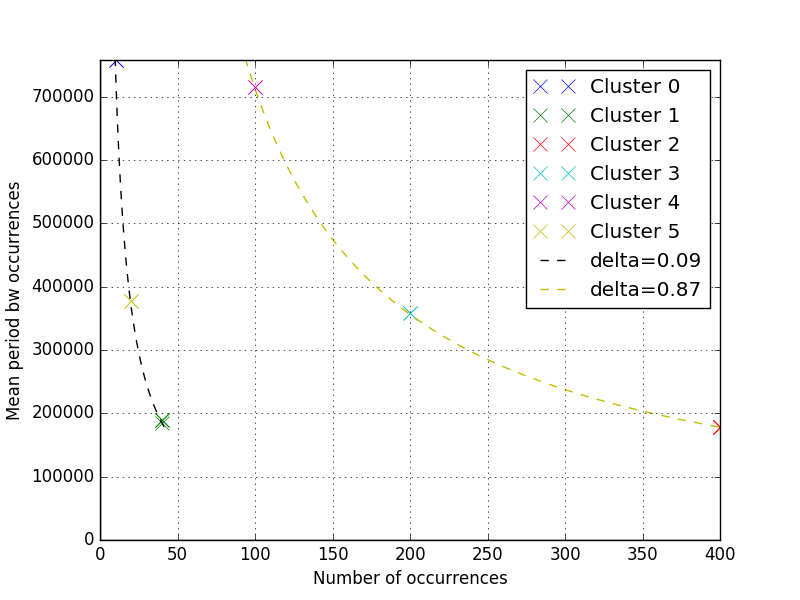
\includegraphics[width=0.5\textwidth]{delta_clustering_test_1}
    \caption{Geometrical representation of delta classification}
    \label{fig:delta_classification_1}
  \end{figure}
  \vfill \null
\end{multicols}

As you can see on figure above, six loops have been detected (this clustering is
related with the previous step not with this last explained delta clustering) 
and classified into two delta groups. The two groups are depicted by these two,
black and yellow curves. So one cluster belongs to one delta if it lies over 
the curve. These curves are described by the function:
$$
f(x)=\frac{\delta*T_{exe}}{x} \text{ being }  0 < \delta \leq 1
$$

Value of $\delta$ is always upper bounder per $1$. It is obvious since one loop
can not have been executed during more time that the entire application time.
Also is lower bounded by zero because if one loop duration is 0 obviously is
would mean it has not been executed. 

Additionally for simplify the loops merging, delta also can be used for
filtering low representative loops. This functionality can be applied even
just after the construction of the $\Omega$ set (reduction step) since at that
point we already have the enough information for calculate $\delta$. Normally,
the lower bound value is set to $0,1$ i.e. It is filtering all loops that
represents less than the 10\% of the overall execution.

On pseudocode \ref{pc:loops_merge_step} there is the actual implementation of
this step. At the very beginning it can be seen how the grouping of the
different loops by deltas is performed, now $\delta$ are subsets of
$\Upsilon$, being $\Delta$ the set of all $\delta$.

\begin{pseudocode}{Loops merge step}{\Upsilon}
\label{pc:loops_merge_step}
    \Delta \GETS deltaClassification(\Upsilon) \\
    \FORALL \delta \in \Delta \DO 
    \BEGIN
        \COMMENT{Sort by it($\upsilon$) desc} \\
        sort(\upsilon \in \delta) \\
        \FOR i \in [0, |\delta|-1) \DO
        \BEGIN
            \FOR j \in [i+1, |\delta|) \DO
            \BEGIN
              \IF isSubloop(\delta_{i}, \delta{j}) \THEN
                  \delta_{i} \mapsto \delta{j} \\
            \END
        \END
    \END
\end{pseudocode}

The key point of this
algorithm is the $isSubloop$ function. Imagine that we have one set of three loops
a, b and c with same $\delta$ with 100, 50 and 10 iterations respectively. 
For sure all three are in a some way related between them but there are two options:
\begin{enumerate*}[label=\roman*)]
    \item $a \mapsto b \mapsto c$
    \item or $a \mapsto c$ and $b \mapsto c$
\end{enumerate*}. You can see the same example where the second option is the
correct on pseudocode
\ref{pc:delta_classification_example_2} and figure
\ref{fig:delta_classification_2}.

\begin{multicols}{2}
  \begin{pseudocode}{Delta example 2}{ }
  \label{pc:delta_classification_example_2}
      \FOR 1 \text{ to } 10 \DO 
      \BEGIN 
        \FOR 1 \text{ to } 5 \DO
        \BEGIN 
            someComms() \\
        \END \\
        \FOR 1 \text{ to } 10 \DO
        \BEGIN 
            someComms()\\
        \END \\
        \text{MPI\_Call} \\
      \END \\
  \end{pseudocode}
  \columnbreak
  \begin{figure}[H]
    \centering
    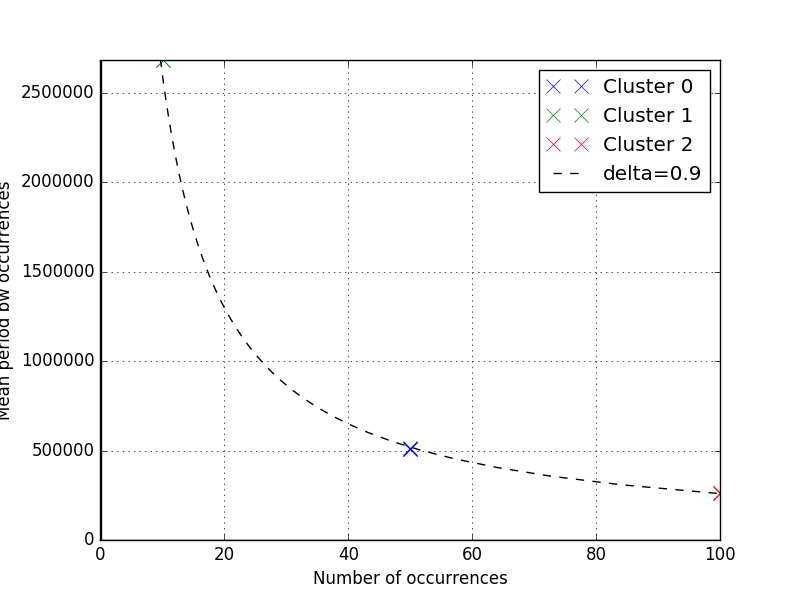
\includegraphics[width=0.5\textwidth]{delta_clustering_test_2}
    \caption{Clustering of delta example 2}
    \label{fig:delta_classification_2}
  \end{figure}
\end{multicols}

In pseudocode \ref{pc:issubloop_function} it can be seen the $isSubloop$ implemented
algorithm.

\begin{pseudocode}{IsSubloop function}{a,b}
\label{pc:issubloop_function}
    \Delta \GETS deltaClassification(\Upsilon) \\
    \FORALL \delta \in \Delta \DO 
    \BEGIN
        \COMMENT{Sort by it($\upsilon$) desc} \\
        sort(\upsilon \in \delta) \\
        \FOR i \in [0, |\delta|-1) \DO
        \BEGIN
            \FOR j \in [i+1, |\delta|) \DO
            \BEGIN
              \IF isSubloop(\delta_{i}, \delta{j}) \THEN
                  \delta_{i} \mapsto \delta{j} \\
            \END
        \END
    \END
\end{pseudocode}

\subsection{Pseudo-code construction}

\chapter{Results}

Some results

\chapter{Conclusions}

Some conclusions



\begin{appendices}
    \chapter{Automatic code instrumentation}\label{ann:automatic_code_instr}

Loops characterization and validation phases of this thesis motivates the development
of an automatization of the user source code instrumentation. It is for sure an
important piece of this thesis but since it is not the main development have been
decided to include it as annex.

As have been previously introduced, this work is done in the Mercurium source-to-source
compiler infrastructure by adding a new phase on the source-to-source compilation workflow
and it basically consists on inject calls to the Extrae API in order to fire events that
\begin{enumerate*}[label=\roman*)]
    \item determine the loops boundaries for the validation
    \item and additionally fire iteration-level metrics to trace for loops characterization
\end{enumerate*}
Further on next sections this process is going to be explained with more details.

\section{Instrumentation for loops characterization}\label{ann:automatic_loops_charac}

\begin{pseudocode}{MonitorLoopInit}{loop_{file}, loop_{line}}
\label{pc:mercurium_monitor_loop_init}
    instrumentLoop \GETS True\\
    \IF size(decissionStack) > 0 \THEN
    \BEGIN
      \COMMENT{Depends on if parent iteration is not instrumented}\\
      instrumentLoop \GETS top(decissionStack)\\
    \END\\
    \IF instrumentLoop \THEN
    \BEGIN
      \COMMENT{Fire loop init event}\\
        ExtraeEvent(LOOPINIT, hash(loop_{file},loop_{line}))\\
        push(iterCounterStack, 0)\\
    \END
\end{pseudocode}

\begin{pseudocode}{MonitorLoopFini}{loop_{file}, loop_{line}}
\label{pc:mercurium_monitor_loop_fini}
    instrumentLoop \GETS True\\
    \IF size(decissionStack) > 0 \THEN
    \BEGIN
      \COMMENT{Depends on if parent iteration is not instrumented}\\
      instrumentLoop \GETS top(decissionStack)\\
    \END\\
    \IF instrumentLoop \THEN
    \BEGIN
      \COMMENT{Fire loop fini event and number of static iterations}\\
        ExtraeEvent(LOOPITERS, pop(iterCounterStack)\\
        ExtraeEvent(LOOPFINI, hash(loop_{file},loop_{line}))\\
    \END
\end{pseudocode}

\begin{pseudocode}{MonitorIterInit}{chance}
\label{pc:mercurium_monitor_iter_init}
    instrumentIter \GETS True\\
    topInstrumentIter \GETS True\\
    r \in U(0,1)\\
    \IF size(decissionStack) > 0 \THEN
    \BEGIN
      \COMMENT{Depends on if parent iteration is not instrumented}\\
      topInstrumentIter \GETS top(decissionStack)\\
    \END\\
    \IF topInstrumentIter \THEN
    \BEGIN
        instrumentIter \GETS (r < chance)\\
        top(iterCounterStack)++\\
        \IF instrumentIter \THEN
        \BEGIN
            \COMMENT{Fire extrae event with HWC attached}\\
            ExtraeEventAndCounters(ITERINIT, top(iterCounterStack))\\
        \END\\
    \END\\
    push(decissionStack, instrumentIter \&  topInstrumentIter)\\
\end{pseudocode}

\begin{pseudocode}{MonitorIterFini}{chance}
\label{pc:mercurium_monitor_iter_fini}
    instrumentIter \GETS pop(decission_stack)\\
    \IF size(decissionStack) > 0 \THEN
    \BEGIN
      \COMMENT{Depends on if parent iteration is not instrumented}\\
      ExtraeEventAndCounters(ITERFINI)
    \END\\
\end{pseudocode}

\subsection{Data quality assesment}\label{ann:loops_data_quality}

In this appendix there will be demonstrated how the degradation of the sampled
data is minimum for different ``chances'' because the high regularity of HPC
applications.

\section{Instrumentation for validation}

Hola manola


\end{appendices}

\bibliography{chapters/bibliography}
\bibliographystyle{apalike}

\end{document}
